\documentclass[11pt,a4paper]{article}

\usepackage[margin=1in]{geometry}
\usepackage{amsmath,amssymb}
\usepackage{booktabs}
\usepackage{graphicx}
\usepackage{xcolor}
\usepackage{hyperref}
\usepackage{caption}
\usepackage{enumitem}
\usepackage{listings}
\usepackage{float}
\usepackage{fancyhdr}
\usepackage{titlesec}
\usepackage{setspace}

\setstretch{1.25}
\setlength{\parskip}{0.4em}
\setlength{\parindent}{0pt}
% تنظیمات لینک‌ها
\hypersetup{
	colorlinks=true,
	linkcolor=blue!50!black,
	citecolor=blue!50!black,
	urlcolor=blue!50!black
}

% تنظیمات نمایش کدها
\lstset{
	basicstyle=\ttfamily\footnotesize,
	breaklines=true,
	columns=fullflexible,
	frame=single,
	backgroundcolor=\color{gray!8},
	xleftmargin=0.5em,
	xrightmargin=0.5em
}

% بسته زی‌پرشین برای پشتیبانی از زبان فارسی
\usepackage{xepersian}
\settextfont{XB Niloofar}
\setlatintextfont{Times New Roman}

% تنظیمات سربرگ و ته‌برگ
\pagestyle{fancy}
\fancyhf{}
\setlength{\headheight}{14pt}
\fancyhead[R]{موتور تشخیص کپی‌های معنایی و سرقت ادبی}
\fancyhead[L]{\thepage}
\renewcommand{\headrulewidth}{0.4pt}

% تنظیمات عنوان‌بندی حرفه‌ای‌تر
\titleformat{\section}
{\Large\bfseries}
{\thesection.}{0.6em}{}

\titleformat{\subsection}
{\large\bfseries}
{\thesubsection.}{0.6em}{}
\begin{document}
	\begin{titlepage}
		\centering
		
		\vspace*{2cm}
		
		{\Huge\bfseries موتور تشخیص کپی‌های معنایی و سرقت ادبی \par}
		
		\vspace{0.8cm}
		
		{\Large \lr{Shingling + MinHash + LSH} و \lr{SimHash} وزن‌دارشده با \lr{TF-IDF} \par}
		
		\vspace{2cm}
		
		{\Large\bfseries پروژه ۳ درس داده‌کاوی \par}
		
		\vspace{0.6cm}
		
		{\large استاد شاکری \par}
		
		\vspace{1.8cm}
		
		{\Large\bfseries اعضای گروه \par}
		
		\vspace{0.8cm}
		
		\begin{tabular}{rl}
			علی تقی‌زاده & ۴۰۳۱۳۰۰۸ \\
			ستایش حاجی اسفندیاری & ۴۰۲۱۳۰۰۸ \\
			زهرا اسلامی‌نیا & ۴۰۲۱۳۰۰۲ \\
		\end{tabular}
		
		\vfill
		


{\large\bfseries لینک مخزن پروژه \par}
\vspace{0.3cm}

{\large
	\href{https://github.com/alitkbbl/Semantic-Plagiarism-Engine}
	{\lr{github.com/alitkbbl/Semantic-Plagiarism-Engine}}
	\par}

\vspace{1cm}
		
	\end{titlepage}
	
	\tableofcontents
	\newpage

	% =========================================================================
	\section{نمای کلی پروژه}
	% =========================================================================
	
	تشخیص اسناد تقریباً تکراری و بازنویسی‌شده، یکی از زیرمسئله‌های اصلی در سامانه‌های تشخیص سرقت ادبی، حذف اخبار تکراری، خوشه‌بندی نتایج جست‌وجو، و تشخیص پرسش‌های تکراری در سامانه‌های پرسش‌وپاسخ \lr{Q\&A} است. دشواری اصلی این مسئله در آن است که اسناد تقریباً تکراری، معمولاً متن \emph{کاملاً یکسان} ندارند. برای نمونه، فردی که مرتکب سرقت ادبی می‌شود ممکن است ترتیب جمله‌ها را تغییر دهد، واژه‌ها را با مترادف‌هایشان جایگزین کند، یا بخش‌هایی از متن را به‌طور کامل بازنویسی نماید؛ با این حال، یک موتور جست‌وجو یا سامانه‌ی تشخیص سرقت ادبی باید همچنان بتواند تشخیص دهد که دو صفحه با بیان‌های متفاوت، محتوای مشابهی را پوشش می‌دهند.
	
	در این پروژه، دو رویکرد کلاسیک و شناخته‌شده برای حل این مسئله پیاده‌سازی و با یکدیگر مقایسه شده‌اند:
	
	\begin{enumerate}
		\item \textbf{روش \lr{Shingling + MinHash + LSH}:}
		در این روش، هر سند به‌صورت مجموعه‌ای از $k$-گرام‌های واژگانی هم‌پوشان، یا همان \lr{shingle}ها، نمایش داده می‌شود. شباهت میان دو سند با استفاده از شاخص \lr{Jaccard} روی این مجموعه‌ها تعریف می‌گردد، سپس این شباهت با کمک امضاهای \lr{MinHash} به‌شکل کارآمد تخمین زده می‌شود. در نهایت، با استفاده از روش \lr{Locality-Sensitive Hashing (LSH)}، جفت‌سندهای کاندیدا پالایش می‌شوند تا در یک پیکره‌ی بزرگ، نیازی به مقایسه‌ی کامل و exhaustive همه‌ی جفت‌ها نباشد.
		
		\item \textbf{روش \lr{TF-IDF Weighted SimHash}:}
		در این روش، هر سند با استفاده از یک فرایند تجمیع هش مبتنی بر علامت و وزن‌دهی‌شده، به یک اثرانگشت \lr{64-bit} تبدیل می‌شود. سپس شباهت میان دو سند، تنها با محاسبه‌ی فاصله‌ی همینگ میان دو عدد با طول ثابت به دست می‌آید.
	\end{enumerate}
	
	هر دو خط لوله فقط با استفاده از کتابخانه‌ی استاندارد \lr{Python}، به‌همراه \lr{NumPy} و \lr{Pandas} پیاده‌سازی شده‌اند. برای الگوریتم‌های اصلی، از هیچ کتابخانه‌ی آماده‌ی \lr{MinHash}، \lr{SimHash} یا \lr{LSH}، مانند \lr{datasketch}، استفاده نشده است. خروجی پروژه به‌صورت یک ابزار خط فرمان با نام \lr{plagiarism\_engine.cli} ارائه شده که شامل سه زیرفرمان \lr{compare}، \lr{corpus} و \lr{pairs} است. برای این پروژه، هیچ رابط گرافیکی یا رابط تعاملی ترمینالی ارائه نشده و چنین رابطی نیز موردنیاز نبوده است.
	
	% =========================================================================
	\section{خط لوله‌ی پیش‌پردازش متن}
	% =========================================================================
	
	پیش از آن‌که هر یک از دو موتور تشخیص شباهت روی متن اعمال شود، همه‌ی اسناد از یک خط لوله‌ی مشترک پیش‌پردازش در فایل \lr{preprocessing.py} عبور می‌کنند:
	
	\begin{enumerate}[label=\arabic*.]
		\item \textbf{نرمال‌سازی نویسه‌ها:}
		ابتدا نرمال‌سازی یونیکد از نوع \lr{NFKC} انجام می‌شود. سپس نویسه‌های مشابه در خط عربی به شکل استاندارد فارسی آن‌ها تبدیل می‌شوند؛ برای مثال، \lr{ARABIC YEH} به \lr{PERSIAN YEH} و \lr{ARABIC KAF} به \lr{PERSIAN KEHEH} نگاشت می‌شود. همچنین حرکات عربی، یا همان \emph{اعراب‌گذاری}، حذف می‌شوند؛ زیرا مشخصات پروژه، علاوه بر انگلیسی، پشتیبانی صحیح از متن فارسی را نیز الزامی کرده است.
		
		\item \textbf{حذف نشانه‌گذاری:}
		هم نشانه‌های نگارشی استاندارد \lr{ASCII} و هم نشانه‌های رایج فارسی/عربی حذف می‌شوند. این نشانه‌ها شامل ویرگول عربی، نقطه‌ویرگول، علامت سؤال، علامت درصد، گیومه‌ها، نویسه‌ی سه‌نقطه، و نویسه‌ی کشیده یا \lr{tatweel/kashida} هستند.
		
		\item \textbf{یکسان‌سازی فاصله‌ها:}
		فاصله‌های متوالی، شامل فاصله‌های معمولی، تب‌ها و شکست‌های خط، به یک فاصله‌ی ساده تبدیل می‌شوند.
		
		\item \textbf{حذف واژه‌های ایست:}
		یک فهرست کوچک و صریح از واژه‌های ایست حذف می‌شود. این فهرست هم واژه‌های انگلیسی مانند \lr{\emph{and}}، \lr{\emph{is}}، \lr{\emph{the}} و \lr{\emph{or}} را پوشش می‌دهد و هم معادل‌های فارسی آن‌ها مانند «و»، «است»، «را» و «یا». در متن انگلیسی اصلی، برخی از این واژه‌های فارسی برای حروف‌چینی به‌صورت لاتین‌نویسی‌شده آمده بودند، اما فهرست واقعی واژه‌های ایست در فایل \lr{preprocessing.py} با خط فارسی ذخیره شده است.
		
		\item \textbf{توکن‌سازی:}
		متن نرمال‌شده بر اساس فاصله‌های خالی به دنباله‌ای از توکن‌ها تبدیل می‌شود.
		
		\item \textbf{ساخت \lr{shingle}:}
		از روی دنباله‌ی توکن‌ها، $k$-گرام‌های واژگانی پیوسته ساخته می‌شوند.
	\end{enumerate}
	
	\subsection{مدیریت حالت‌های مرزی}
	
	در مشخصات پروژه، سه حالت مرزی به‌صورت صریح مطرح شده است. هر سه حالت، هم با سندهای اختصاصی در مسیر \lr{data/sample\_corpus/} و هم با آزمون‌های واحد در فایل \lr{tests/test\_engine.py} بررسی شده‌اند:
	
	\begin{itemize}
		\item \textbf{اسناد خالی} \lr{(doc\_09.txt):}
		سندهای خالی به‌جای آن‌که باعث ایجاد استثنا شوند، یک فهرست توکن خالی و یک مجموعه‌ی \lr{shingle} خالی تولید می‌کنند. طبق قرارداد، دو سند خالی مشابهت کامل دارند و مقدار $J = 1.0$ برای آن‌ها در نظر گرفته می‌شود. این تصمیم با قرارداد رایج برای حالت نامعین $0/0$ در شباهت \lr{Jaccard} سازگار است.
		
		\item \textbf{اسناد بسیار کوتاه} \lr{(doc\_07.txt}، شامل پنج واژه\lr{):}
		اگر تعداد توکن‌های یک سند از اندازه‌ی پیکربندی‌شده‌ی \lr{shingle} یعنی $k$ کمتر باشد، به‌جای آن‌که هیچ \lr{shingle}ای تولید نشود، کل دنباله‌ی توکن‌ها به‌عنوان یک \lr{shingle} واحد در نظر گرفته می‌شود. به این ترتیب، سندهای کوتاه همچنان قابل مقایسه باقی می‌مانند.
		
		\item \textbf{نویسه‌های غیرمعمول} \lr{(doc\_08.txt):}
		شامل ایموجی، حروف لاتین دارای اعراب، خط تیره‌ی بلند، نقل‌قول‌های خمیده:
		همه‌ی نویسه‌های کنترلی، قالب‌بندی و جانشین یونیکد حذف می‌شوند. در عین حال، نویسه‌های فاصله با دقت حفظ می‌شوند، هرچند از نظر رده‌بندی عمومی یونیکد در همان خانواده قرار می‌گیرند. این کار باعث می‌شود ورودی‌های ناسالم یا بدقالب، باعث توقف خط لوله یا تخریب مرزهای \lr{shingle} نشوند.
	\end{itemize}
	
	% =========================================================================
	\section{روش اول: \lr{Shingling + MinHash + LSH}}
	% =========================================================================
	
	\subsection{شباهت دقیق \lr{Jaccard} و هزینه‌ی آن}
	
	اگر دو مجموعه‌ی \lr{shingle} را با $A$ و $B$ نشان دهیم، شباهت \lr{Jaccard} به‌صورت زیر تعریف می‌شود:
	$$
	J(A, B) = \frac{|A \cap B|}{|A \cup B|}.
	$$
	این معیار به‌صورت مستقیم در فایل \lr{cli.py} و در تابع \lr{\_exact\_jaccard} پیاده‌سازی شده است. از این مقدار هم به‌عنوان سیگنال مرجع برای راستی‌آزمایی استفاده می‌شود و هم به‌عنوان معیاری که \lr{MinHash} برای تقریب آن طراحی شده است.
	
	\paragraph{چرا مقایسه‌ی دقیق جفت‌به‌جفت از مرتبه‌ی $O(n^2)$ است؟}
	برای یک پیکره شامل $n$ سند، یافتن \emph{همه‌ی} جفت‌هایی که شباهتشان از یک آستانه‌ی مشخص بیشتر است، در روش ساده نیازمند محاسبه‌ی $J(A,B)$ برای تمام جفت‌های نامرتب اسناد است. تعداد این جفت‌ها برابر است با:
	$$
	\binom{n}{2} = \frac{n(n-1)}{2}.
	$$
	هر محاسبه‌ی منفرد \lr{Jaccard} با استفاده از اشتراک‌گیری مجموعه‌های هش‌شده، هزینه‌ای در حد $O(|A| + |B|)$ دارد؛ اما تعداد \emph{جفت‌ها} همچنان با $n$ به‌صورت درجه‌دو رشد می‌کند. بنابراین، دو برابر شدن اندازه‌ی پیکره تقریباً باعث چهار برابر شدن تعداد مقایسه‌های موردنیاز می‌شود. برای پیکره‌ی نمونه‌ی ۱۱ سندی این پروژه، این مقدار فقط ۵۵ مقایسه است و ناچیز محسوب می‌شود؛ اما در یک سامانه‌ی واقعی تشخیص سرقت ادبی که مثلاً $n = 100{,}000$ سند را پردازش می‌کند، مقایسه‌ی کامل به حدود $5 \times 10^9$ مقایسه‌ی جفتی نیاز دارد. اجرای تکرارشونده‌ی چنین حجمی از مقایسه، از نظر محاسباتی عملی نیست. دقیقاً همین مسئله‌ی مقیاس‌پذیری است که ترکیب \lr{MinHash + LSH} برای دور زدن آن طراحی شده است.
	
	\subsection{\lr{MinHash}، پیاده‌سازی‌شده از پایه}
	
	روش \lr{MinHash} که توسط \lr{Broder} در سال \lr{1997} معرفی شد، از یک واقعیت احتمالاتی ساده استفاده می‌کند: اگر $h$ یک تابع هش تصادفی یکنواخت از خانواده‌ای مناسب باشد، آنگاه:
	$$
	\Pr\big[\min_{x \in A} h(x) = \min_{x \in B} h(x)\big] = J(A, B).
	$$
	با انتخاب $\text{num\_perm}$ تابع هش مستقل و ثبت کمترین مقدار هش روی مجموعه‌ی \lr{shingle}های هر سند برای هر تابع، یک \emph{امضا} با طول ثابت ساخته می‌شود. سپس نسبت جایگاه‌هایی از امضای دو سند که مقدار یکسان دارند، یک برآوردگر بدون اریب برای شباهت واقعی \lr{Jaccard} است. خطای استاندارد این برآوردگر با نرخ $O(1/\sqrt{\text{num\_perm}})$ کاهش می‌یابد.
	
	\paragraph{جزئیات پیاده‌سازی.}
	فایل \lr{minhash.py} خانواده‌ی استاندارد هش همگانی زیر را پیاده‌سازی می‌کند:
	$$
	h_i(x) = (a_i \cdot x + b_i) \bmod p, \qquad p = 2^{61} - 1
	$$
	که در آن $p$ یک عدد اول \lr{Mersenne} است. ضرایب $(a_i, b_i)$ برای هر نمونه از \lr{MinHasher} فقط یک‌بار و با استفاده از یک مولد تصادفی دارای بذر مشخص تولید می‌شوند. از آن‌جا که تابع داخلی \lr{hash()} در \lr{Python} به دلایل امنیتی و از طریق \lr{PYTHONHASHSEED} در هر فرایند مقداردهی تصادفی می‌شود، نمی‌توان از آن برای نگاشت رشته‌های \lr{shingle} به عدد صحیح استفاده کرد. در \lr{MinHash}، یک \lr{shingle} یکسان باید در همه‌ی اسناد و در همه‌ی اجراها هش یکسانی داشته باشد. به همین دلیل، ابتدا از \lr{SHA-1}، کوتاه‌شده به \lr{64} بیت، به‌عنوان هش پایه‌ی پایدار در تابع \lr{stable\_hash} استفاده شده و سپس خانواده‌ی هش همگانی روی آن عدد اعمال شده است.
	
	اگر مجموعه‌ی \lr{shingle} یک سند خالی باشد، امضایی شامل مقدار نگهبان بیشینه برای همه‌ی خانه‌ها تولید می‌شود. بنابراین، دو سند خالی مشابه یکدیگر در نظر گرفته می‌شوند که با قرارداد شباهت \lr{Jaccard} در بخش قبل سازگار است.
	
	\subsection{\lr{LSH} مبتنی بر باند، پیاده‌سازی‌شده از پایه}
	
	یک امضای \lr{MinHash} با طول \lr{num\_perm} به \lr{num\_bands} باند پیوسته تقسیم می‌شود. تعداد ردیف‌های هر باند برابر است با:
	$$
	r = \text{num\_perm} / \text{num\_bands}.
	$$
	هر باند با استفاده از \lr{SHA-1} روی مقادیر خام امضا هش می‌شود. همچنین شاخص باند به‌عنوان نمک به هش افزوده می‌شود تا اگر مقادیر ردیف‌ها در دو باند متفاوت یکسان بودند، به‌اشتباه با یکدیگر برخورد نکنند. دو سند فقط زمانی به‌عنوان \emph{کاندیدا} برای مقایسه‌ی دقیق‌تر در نظر گرفته می‌شوند که دست‌کم یکی از باندهای آن‌ها در یک سطل مشترک قرار گیرد.
	
	\paragraph{چرا این روش تعداد مقایسه‌ها را کاهش می‌دهد؟}
	در این روش، فقط سندهایی که در یک سطل مشترک برخورد کرده‌اند با معیار دقیق \lr{Jaccard} مقایسه می‌شوند. سندهایی که هیچ باند مشترکی ندارند، اساساً وارد مجموعه‌ی کاندیداها نمی‌شوند. بخش~\ref{sec:results} کاهش واقعی به‌دست‌آمده روی پیکره‌ی نمونه را گزارش می‌کند: کاهش \lr{94.55\%}، یعنی فقط ۳ جفت از ۵۵ جفت ممکن وارد مرحله‌ی راستی‌آزمایی شدند.
	
	\paragraph{منحنی \lr{S} و انتخاب پارامتر.}
	طرح باندبندی، رابطه‌ی مشهور «منحنی \lr{S}» را میان شباهت واقعی \lr{Jaccard} یک جفت سند، یعنی $s$، و احتمال کاندیدا شدن آن جفت ایجاد می‌کند:
	$$
	P(\text{candidate} \mid s) = 1 - (1 - s^r)^b.
	$$
	این رابطه در فایل \lr{lsh.py} و در تابع \lr{candidate\_probability} پیاده‌سازی شده است. مقدار این تابع برای $s$های پایین‌تر از یک آستانه، نزدیک به صفر و برای $s$های بالاتر از آن آستانه، نزدیک به یک است. تندترین ناحیه‌ی گذار آن تقریباً در نقطه‌ی زیر رخ می‌دهد:
	$$
	s^{*} = \Big(\frac{1}{b}\Big)^{1/r}
	$$
	که در تابع \lr{s\_curve\_threshold} محاسبه می‌شود. شکل~\ref{fig:s-curve} این منحنی را برای سه تقسیم‌بندی متفاوت \lr{(num\_bands, rows\_per\_band)} از یک امضای \lr{MinHash} با \lr{128} جایگشت نشان می‌دهد.
	
	تعداد باندهای کمتر با اندازه‌ی بزرگ‌تر، مانند $b=8, r=16$، آستانه‌ی گذار را بالاتر می‌برد. این حالت باعث تولید کاندیداهای مثبت کاذب کمتر می‌شود، اما منحنی آن تندتر و کم‌گذشت‌تر است و ممکن است جفت‌های با شباهت متوسط را از دست بدهد. در مقابل، تعداد باندهای بیشتر با اندازه‌ی کوچک‌تر، مانند $b=32, r=4$، آستانه‌ی گذار را پایین‌تر می‌آورد. این حالت شباهت‌های ضعیف‌تر را نیز پیدا می‌کند، اما در عوض جفت‌های کاندیدای بیشتری تولید می‌شود که باید در مرحله‌ی بعد با معیار دقیق بررسی شوند. بنابراین، انتخاب باندها یک مصالحه‌ی مستقیم و قابل تنظیم میان بازیابی در مرحله‌ی تولید کاندیدا و هزینه‌ی محاسباتی مرحله‌ی راستی‌آزمایی است.
	
	\begin{figure}[H]
		\centering
		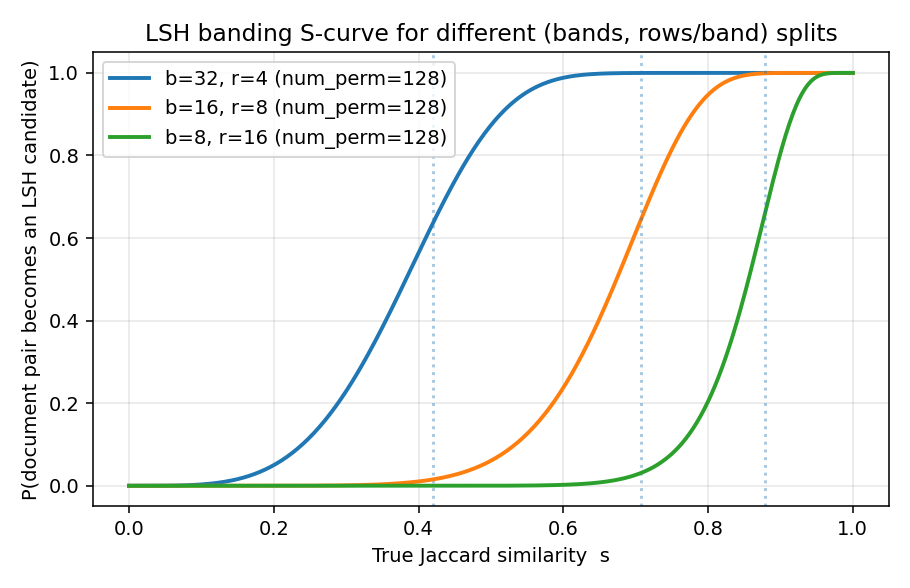
\includegraphics[width=0.72\textwidth]{figures/lsh_s_curve.png}
		\caption{منحنی \lr{S} در روش باندبندی \lr{LSH} برای سه پیکربندی مختلف \lr{(bands, rows-per-band)} از یک امضای \lr{MinHash} با \lr{128} جایگشت. خط‌های عمودی نقطه‌چین، آستانه‌ی تقریبی تشخیص هر پیکربندی را نشان می‌دهند:
			$s^{*} = (1/b)^{1/r}$.}
		\label{fig:s-curve}
	\end{figure}
	
	
	% =========================================================================
	\section{روش دوم: \lr{SimHash} وزن‌دهی‌شده با \lr{TF-IDF}}
	% =========================================================================
	
	الگوریتم \lr{SimHash} (Charikar, 2002) رویکرد متفاوتی را اتخاذ می‌کند: به جای آنکه یک سند را به عنوان یک \emph{مجموعه} در نظر بگیرد، یک اثرانگشت (fingerprint) واحد با طول ثابت را به گونه‌ای انباشت می‌کند که اسناد مشابه در فاصله همینگ (Hamming distance) کوچکی از یکدیگر قرار گیرند. این کار، جستجوی شباهت را به یک شمارش بیتِ ساده تبدیل می‌کند.
	
	\subsection{الگوریتم.} برای سندی که به صورت یک کیسهٔ کلماتِ وزن‌دار (weighted bag of tokens) به فرم $\{(\text{\lr{term}}, w)\}$ نمایش داده می‌شود:
	\begin{enumerate}[label=\arabic*.]
		\item یک انباشتگر ۶۴-بعدی $V = \mathbf{0}$ را مقداردهی اولیه کنید.
		\item برای هر ترم (term)، یک هشِ ۶۴-بیتی پایدار از آن محاسبه کنید (در اینجا از \lr{BLAKE2b} استفاده شده است تا از تابع درونی و تصادفی \lr{\texttt{hash()}} در پایتون اجتناب شود).
		\item برای هر یک از ۶۴ موقعیت بیتی $i$: اگر بیت $i$ام از هشِ ترم برابر با $1$ بود، وزن $w$ مربوط به آن ترم را به $V_i$ اضافه کنید؛ در غیر این صورت، $w$ را از $V_i$ کم کنید.
		\item در نهایت، بیت $i$امِ اثرانگشت برابر با $1$ خواهد بود اگر $V_i > 0$ باشد، و در غیر این صورت برابر با $0$ است.
	\end{enumerate}
	وزن $w$ برای هر ترم برابر با امتیاز \lr{TF-IDF} آن است که از پایه در کلاس \lr{\texttt{TfidfVectorizerFromScratch}} و با استفاده از فرمول استانداردِ هموارشده (smoothed) زیر محاسبه می‌گردد:
	$$
	\mathrm{idf}(t) = \ln\!\left(\frac{1+N}{1+\mathrm{df}(t)}\right) + 1,
	$$
	به این ترتیب، ترمی که در \emph{تمامی} اسنادِ پیکرهٔ آموزش‌دیده (fitted corpus) ظاهر می‌شود، به جای وزنِ دقیقاً صفر، همچنان یک وزن مثبت کوچک دریافت می‌کند و ترم‌های دیده‌نشده در زمان استنتاج، به طور منطقی به بیشینهٔ مقدار \lr{IDF} در پیکره بازمی‌گردند. شباهت بین دو اثرانگشت، هم به صورت فاصله همینگ خام (\lr{\texttt{hamming\_distance}}) و هم به صورت یک شباهت نرمال‌شده در بازه $[0,1]$ (\lr{\texttt{hamming\_similarity}} $= 1 - d_H / 64$) گزارش می‌شود.
	
	\subsection{چرا وزن‌دهی \lr{TF-IDF} اهمیت دارد.} در یک \lr{SimHash} بدون وزن‌دهی (وزن برابر برای همهٔ توکن‌ها)، کلمات رایج با اطلاعات کم می‌توانند بر اثرانگشت غلبه کنند و اثر آن را مخدوش سازند. وزن‌دهیِ مشارکت هر ترم بر اساس میزان کمیابیِ آن در سطح پیکره، قدرت تمایزِ اثرانگشت را بر روی کلماتی متمرکز می‌کند که در واقعیت موضوع یک سند را از سند دیگر متمایز می‌سازند -- این رویکرد معادلِ پیوسته (و نه باینری) برای حذف کلمات توقف (stop-word removal) در فضای \lr{SimHash} است.
	
	% =========================================================================
	\section{انتخاب پارامترها}
	\label{sec:params}
	% =========================================================================
	
	\subsection{اندازه شینگل ($k$)}
	\label{sec:shingle-size-short}
	
	مشخصات پروژه مقادیر $k \in \{3, 4, 5\}$ را برای شینگل‌بندی (shingling) توصیه می‌کند. این توصیه به طور ضمنی فرض می‌کند که اسناد در حد و اندازهٔ یک پاراگراف هستند؛ به عنوان مثال، برای اسناد نمونهٔ پاراگرافی در مسیر \lr{\texttt{data/sample\_corpus/}} (هر کدام شامل ۵۰ تا ۷۵ توکن)، مقدار $k=3$ مجموعه‌های شینگلی ایجاد می‌کند که به اندازه کافی بزرگ هستند (۵۰ تا ۷۰ شینگل در هر سند) تا سیگنال پایداری برای \lr{MinHash} فراهم کنند، در حالی که همچنان به ویرایش‌های سطح کلمه حساس باقی می‌مانند.
	
	متن‌های کوتاه در حد یک جمله رفتار بسیار متفاوتی دارند. جدول~\ref{tab:threshold-sweep} جاروب آستانه (threshold sweep) را برای بهترین امتیاز \lr{F1} قابل دستیابی در اندازه‌های مختلف شینگل بر روی مجموعه دادهٔ مصنوعی جفت-پرسش (بخش~\ref{sec:pairs-dataset}) نشان می‌دهد؛ جایی که هر سند تنها یک پرسشِ $\sim$۱۰ کلمه‌ای است: با استفاده از شینگل‌های $k=3$، تنها ۶ تا ۹ شینگل به ازای هر سند باقی می‌ماند، بنابراین جایگزینیِ تنها یک کلمه می‌تواند به طور مستقیم بخش عمده‌ای از شینگل‌های یک سند را از بین ببرد و سیگنال ژاکارد (Jaccard) را تخریب کند. کاهش $k$ به $1$ (یعنی همان اشتراک کلمات ساده بر اساس ژاکارد)، سیگنال بسیار بیشتری را برای اسناد کوتاه بازیابی می‌کند. \textbf{بنابراین، ما از $k=3$ به عنوان مقدار پیش‌فرض برای دستورات \lr{\texttt{compare}}/\lr{\texttt{corpus}} (اسناد پاراگرافی) و از $k=1$ برای اجرای نمونهٔ \lr{\texttt{pairs}} بر روی مجموعه دادهٔ کوتاه (پرسشی) استفاده می‌کنیم}، و پرچم \lr{\texttt{--shingle-size}} را در رابط خط فرمان (CLI) قرار داده‌ایم تا بتوان آن را برای طول معمول اسناد در پیکرهٔ هدف تنظیم کرد.
	
	\begin{table}[H]
		\centering
		\caption{بهترین مقدار \lr{F1} قابل دستیابی (از طریق جاروب آستانه) بر روی مجموعه داده مصنوعی جفت-پرسش، بر اساس روش و اندازهٔ شینگل. اندازه‌های کوچکتر شینگل، سیگنال بیشتری را برای اسناد کوتاه و جمله‌ای بازیابی می‌کنند.}
		\label{tab:threshold-sweep}
		\begin{tabular}{@{}llrrr@{}}
			\toprule
			\lr{Method} & \lr{Config} & \lr{Best threshold} & \lr{Precision} & \lr{Recall / F1} \\
			\midrule
			\lr{MinHash+LSH} & $k=1$ & $0.13$ & $0.730$ & $0.900\ /\ 0.806$ \\
			\lr{MinHash+LSH} & $k=2$ & $0.01$ & $0.697$ & $0.767\ /\ 0.730$ \\
			\lr{MinHash+LSH} & $k=3$ & $0.01$ & $0.783$ & $0.600\ /\ 0.679$ \\
			\lr{TF-IDF SimHash} & \lr{64-bit} & $0.46$ & $0.556$ & $1.000\ /\ 0.714$ \\
			\bottomrule
		\end{tabular}
	\end{table}
	
	\subsection{طول امضای \lr{MinHash} (\lr{\texttt{num\_perm}})}
	
	مشخصات مسئله، ۱۲۸ یا ۲۵۶ جایگشت (permutation) را توصیه می‌کند. خطای استانداردِ تخمینِ ژاکارد در \lr{MinHash} تقریباً برابر با $1/\sqrt{\text{\lr{num\_perm}}}$ است: حدود $8.8\%$ برای ۱۲۸ جایگشت، و حدود $6.25\%$ برای ۲۵۶ جایگشت. ما از مقدار \textbf{۱۲۸} به عنوان پیش‌فرض استفاده می‌کنیم که تعادل منطقی و مناسبی بین دقت و هزینهٔ محاسبهٔ امضا (هر جایگشت اضافی به معنای یک اسکنِ کمینه (min-scan) با مرتبه $O(|\text{\lr{shingles}}|)$ به ازای هر سند است) برای پروژه‌ای با این مقیاس ارائه می‌دهد؛ با این حال، پارامتر \lr{\texttt{--num-perm}} در دسترس است تا هر کسی که دقت بالاتری (۲۵۶ جایگشت) را با دو برابر هزینه می‌خواهد، بتواند آن را تنظیم کند.
	
	\subsection{باندهای \lr{LSH} (\lr{\texttt{num\_bands}})}
	
	با فرض $\text{\lr{num\_perm}}=128$، پیش‌فرض ما $\text{\lr{num\_bands}}=32$ (که نتیجه می‌دهد $r=4$ سطر در هر باند) است. این مقادیر آستانهٔ تشخیص تقریبی برابر با $s^{*} = (1/32)^{1/4} \approx 0.42$ را به دست می‌دهند (شکل~\ref{fig:s-curve}). این مقدار به صورت تجربی به گونه‌ای انتخاب شد که به اندازه کافی پایین باشد تا به طور پایدار و قابل‌اطمینان حالتِ ``تکثیرِ تقریبی خفیف (light near-duplicate)'' را در پیکرهٔ نمونه (فایل \lr{\texttt{doc\_01.txt}} در برابر \lr{\texttt{doc\_11.txt}} با مقدار واقعی ژاکارد $\approx 0.48$) به عنوان یک کاندیدای \lr{LSH} نشان دهد، و همزمان به اندازه کافی بالا باشد تا اسناد کاملاً نامرتبط اساساً هیچ‌گاه به طور تصادفی با هم تداخل (collide) نداشته باشند.
	
	\subsection{عرض بیت \lr{SimHash}}
	
	بر اساس مشخصات، بر روی ۶۴ بیت ثابت شده است. ۶۴ بیت همچنین اندازهٔ کلمه ماشین (machine word size) در تقریباً تمامی سخت‌افزارهای مدرن است که باعث می‌شود محاسبهٔ فاصله همینگ (به شکل \lr{\texttt{bin(a \textasciicircum{} b).count("1")}}) کم‌هزینه و سریع باقی بماند.
	
	\subsection{آستانه‌های تصمیم‌گیری}
	
	آستانهٔ شباهت در تمامی دستورات خط فرمان به جای هاردکد شدن، به عنوان یک پرچم در دسترس قرار گرفته است (\lr{\texttt{--threshold}} برای \lr{\texttt{corpus}}، و \lr{\texttt{--minhash-threshold}} / \lr{\texttt{--simhash-threshold}} برای \lr{\texttt{pairs}})، زیرا همان‌طور که جدول~\ref{tab:threshold-sweep} نشان می‌دهد، نقطهٔ عملیاتیِ درست به شدت وابسته به طول سند و هزینهٔ نسبی مثبت کاذب در برابر منفی کاذب در بستر استقرار (deployment context) است (به عنوان مثال، یک ابزار تشخیص سرقت ادبی که برای ارجاع کار به بررسیِ \emph{انسانی} استفاده می‌شود، می‌تواند نقطهٔ عملیاتی با دقت پایین‌تر و فراخوانی بالاتری را نسبت به ابزاری که اقدام خودکار انجام می‌دهد، تحمل کند).
	
	\subsection{انتخاب خودکار آستانه (\lr{\texttt{--sweep}})}
	\label{sec:sweep}
	
	حدس زدن دستیِ یک آستانه و امید به اینکه این مقدار بر روی یک مجموعه دادهٔ جدید نیز جواب دهد، در عمل آن‌قدر غیرقابل اعتماد بود که توجیه می‌کرد به جای یک اسکریپت تحلیلِ یک‌بارمصرف، به عنوان یک قابلیت اصلی در ابزار پشتیبانی شود. \\
	دستور \lr{\texttt{pairs}} پرچم \lr{\texttt{--sweep}} را می‌پذیرد: \\
	 امتیاز شباهتِ هر جفت دقیقاً یک بار محاسبه می‌شود و سپس در یک شبکه (پنجرهٔ) آستانه‌ها (به طور پیش‌فرض: $0.00$ تا $1.00$ با گام‌های $0.02$) از طریق تابع \lr{\texttt{sweep\_thresholds}} مجدداً ارزیابی می‌شود، و آستانه‌ای که \lr{F1} را بیشینه می‌کند توسط \lr{\texttt{best\_threshold\_row}} انتخاب می‌گردد. از آنجایی که بخش عمدهٔ هزینه مربوط به امتیازدهی است و اعمال مجدد آستانه‌ها بر روی لیست امتیازاتِ از پیش محاسبه شده از مرتبه $O(1)$ به ازای هر آستانه است، یک جاروبِ کامل به سختی هزینه‌ای بیشتر از یک اجرایِ تک‌آستانه‌ای دارد. آستانهٔ انتخاب شده در خروجی (ستون \lr{\texttt{threshold\_used}}) ثبت می‌شود تا نتایج قابل تکرار باقی بمانند، و پرچم \lr{\texttt{--sweep-output}} می‌تواند کل منحنی دقت/فراخوانی/\lr{F1} بر حسب آستانه را برای تحلیل‌های بعدی ذخیره کند (شکل~\ref{fig:threshold-sweep-curve}).
	
	\begin{figure}[H]
		\centering
		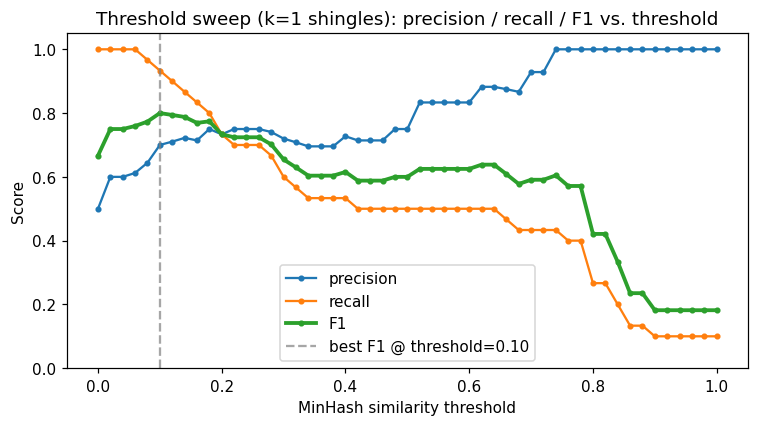
\includegraphics[width=0.72\textwidth]{figures/threshold_sweep_curve.png}
		\caption{دقت، فراخوانی و \lr{F1} به عنوان تابعی از آستانهٔ شباهت \lr{MinHash} ($k=1$)، جاروب‌شده بر روی مجموعه داده مصنوعی برچسب‌دار جفت‌ها. خط‌چین نشان‌دهنده آستانه بیشینه‌کننده \lr{F1} است که دستور \lr{\texttt{--sweep}} به صورت خودکار انتخاب می‌کند.}
		\label{fig:threshold-sweep-curve}
	\end{figure}
	
	این قابلیت به طور خاص در پاسخ به یک خطای واقعی در هنگام ارزیابی روی \lr{PAN-PC-11} (بخش~\ref{sec:pan-pc11-results}) اضافه شد: آستانه‌های پیش‌فرض ثابتی که برای یک نوع متن تنظیم شده بودند، \emph{دقتی تقریباً بی‌نقص اما فراخوانیِ کاملاً فروپاشیده‌ای} روی نوع دیگری از متن تولید کردند. این یک الگوی تشخیصی است که ارزش نام‌گذاری صریح را دارد، زیرا به راحتی ممکن است با معیوب بودنِ معیار شباهت اشتباه گرفته شود، در حالی که مشکل تنها به کالیبره نبودنِ مرز تصمیم برمی‌گردد. در صورت وجود هرگونه آستانهٔ قابل استفاده، جاروب کردن این مشکل را حل می‌کند؛ بخش~\ref{sec:pan-pc11-results} همچنین موردی را مستند می‌کند که در آن جاروب آستانه نشان می‌دهد \emph{هیچ} آستانه‌ای نمی‌تواند از خط‌پایهٔ بدیهی و پیش‌پاافتادهٔ ``همیشه پیش‌بینی کن تکراری است'' بهتر عمل کند، که این خود اطلاعاتی تشخیصی درباره انتخاب هایپرپارامترها محسوب می‌شود، نه خرابیِ ابزار.
	
	\subsection{بازبینی اندازه شینگل: بازه‌های طولانی و مبهم (\lr{PAN-PC-11})}
	\label{sec:shingle-size-pan}
	
	بخش~\ref{sec:shingle-size-short} نشان داد که پرسش‌های کوتاه به اندازه شینگل کوچکتری نسبت به $k \in \{3,4,5\}$ که در مشخصات توصیه شده نیاز دارند، زیرا اساساً متنِ کافی برای تشکیل شینگل‌های زیاد وجود ندارد. مجموعه داده واقعی \lr{PAN-PC-11} (بخش~\ref{sec:pan-pc11-dataset}) نیز به دلیلی \emph{دقیقاً متضاد}، همین نتیجه یعنی $k=1$ را ایجاب می‌کند: بازه‌های سرقت ادبی در آن طولانی هستند (طول بازه‌های حاشیه‌نویسی‌شدهٔ مشاهده‌شده از ۱,۴۲۱ تا ۱۸,۰۰۶ کاراکتر متغیر بود) اما مکرراً از طریق پخش کردنِ جایگزینی‌ها در سطح کلمه در سراسر متن، به جای بازنویسی عبارات متصل، \emph{مبهم‌سازی (obfuscated)} شده‌اند. جایگزینیِ تنها یک کلمه، تمام شینگل‌های $k$-کلمه‌ای متداخل با آن را از بین می‌برد؛ در طول یک بازه طولانی با تعداد زیادی از این جایگزینی‌های پراکنده، این اثر انباشته می‌شود و می‌تواند اکثر اشتراکات واقعی را پاک کند، با وجود اینکه اکثریت قاطعِ واژگانِ متن همچنان مشترک هستند. شینگل‌بندی تک‌کلمه‌ای (که در عمل معادل استفاده از روش ژاکارد با کیسه-کلمات ساده است) نسبت به \emph{مکان} وقوع یک ویرایش تا حد زیادی بی‌تفاوت است، هرچند که هزینهٔ آن از دست دادن کامل آزمونِ ترتیب محلی کلمات خواهد بود. جدول~\ref{tab:pan-pc11-results} تفاوت حاصل از این مسئله را به صورت کمی نشان می‌دهد: بر روی همان مجموعه ارزیابی ۴,۰۰۰ جفتی، برای \lr{MinHash+LSH}، مقدار $F_1$ از $0.070$ در $k=3$ (آستانه‌های ثابت) به $0.920$ در $k=1$ (آستانه جاروب‌شده) افزایش می‌یابد. \textbf{بنابراین، ما اندازهٔ شینگل را به عنوان یک هایپرپارامتر وابسته به پیکره در نظر می‌گیریم که باید به ازای هر استقرار تنظیم شود، نه یک ثابت غیرقابل تغییر} -- مقدار $k=3$ به عنوان پیش‌فرضی مناسب برای اسناد پاراگرافی، در دستورات \lr{\texttt{compare}}/\lr{\texttt{corpus}} باقی می‌ماند، اما به محض استفاده از داده‌های واقعی، هر دو ارزیابی انجام شده در این گزارش نیازمند مقدار کوچکتری بودند.
	
	
	% =========================================================================
	\section{مجموعه‌داده‌ها}
	\label{sec:pairs-dataset}
	% =========================================================================
	
	\subsection{مجموعه‌داده‌های مقیاس‌بزرگِ پیشنهادی (غیرموجود در مخزن)}
	
	بر اساس مشخصات پروژه، مجموعه‌داده‌های خام و حجیم در این مخزن گنجانده \emph{نشده‌اند}. فایل \lr{\texttt{data/raw/README.md}} نحوه‌ی دریافت و اتصال هر یک از سه مجموعه‌داده‌ی پیشنهادی زیر را مستند کرده است:
	
	\begin{itemize}
		\item \textbf{پیکره‌ی \lr{PAN-PC-11} (پیکره‌ی سرقت ادبی \lr{PAN} سال ۲۰۱۱):} مجموعه‌داده‌ی پیشنهادی اصلی که شامل موارد سرقت ادبی با مبهم‌سازی (Obfuscation) دستی و خودکار است و از طریق پلتفرم \lr{Zenodo} در دسترس قرار دارد.
		\item \textbf{اسناد تکراری \lr{Stack Exchange}:} جفت‌پست‌های پرسش‌وپاسخ که به‌عنوان تکراری برچسب‌گذاری شده‌اند و در هاب \lr{Hugging Face} موجود هستند.
		\item \textbf{جفت‌محورهای پرسش \lr{Quora}:} شامل بیش از $400{,}000$ جفت پرسش با برچسب تکراری / غیرتکراری که در هاب \lr{Hugging Face} و \lr{Kaggle} قابل دسترسی است.
	\end{itemize}
	
	\subsection{پیکره‌ی نمونه (\lr{\texttt{data/sample\_corpus/}})}
	
	یک پیکره‌ی ۱۱ سندی به‌صورت دستی نگارش شد تا تمامی حالات بررسی‌شده در این گزارش را به‌طور هم‌زمان بیازماید:
	یک پاراگراف مرجع در مورد انرژی‌های تجدیدپذیر (\lr{\texttt{doc\_01.txt}}) به همراه یک کپی واژه‌به‌واژه و عینی از آن (\lr{\texttt{doc\_03.txt}}، شبیه‌سازی سرقت ادبی از نوع کپی-پیست)، یک نسخه‌ی تقریباً تکراری با ویرایش جزئی (\lr{\texttt{doc\_11.txt}}، جایگزینی‌های جزئی کلمات)، و یک نسخه‌ی تقریباً تکراری با بازنویسی سنگین (\lr{\texttt{doc\_02.txt}}، بازنویسی کامل)؛ یک پاراگراف مرجع دوم و نامرتبط در مورد اکتشاف مریخ (\lr{\texttt{doc\_04.txt}}) به همراه نسخه‌ی بازنویسی‌شده‌ی سنگینِ خاص خود (\lr{\texttt{doc\_05.txt}})؛ یک پاراگراف نامرتبط در حوزه‌ی آشپزی (\lr{\texttt{doc\_06.txt}})؛ و چهار سند مربوط به حالات مرزی (اسناد بسیار کوتاه، نویسه‌های غیرمعمول، سند خالی، و متن به زبان فارسی).
	
	\subsection{مجموعه‌داده‌ی مصنوعیِ جفت‌های برچسب‌دار (\lr{\texttt{data/raw/quora/sample\_pairs.csv}})}
	
	از آنجا که محیط بیلد مورد استفاده برای تهیه این گزارش دسترسی به شبکه نداشت، امکان دانلود مجموعه‌داده‌ی واقعی جفت‌محورهای پرسش \lr{Quora} فراهم نبود. بنابراین، یک مجموعه‌داده‌ی مصنوعی ۶۰ سطری با همان ساختار و شمای استاندارد (\lr{\texttt{question1, question2, is\_duplicate}}) به‌صورت دستی ایجاد شد تا فرمان \lr{\texttt{pairs}} بدون نیاز به هیچ پیکربندی اضافی قابل اجرا و ارزیابی باشد. این مجموعه‌داده به‌طور تعمدی چهار سطح از دشواری را پوشش می‌دهد (هر کدام ۱۵ جفت، مگر مواردی که ذکر شده است):
	
	\begin{itemize}
		\item \textbf{تکراری‌های آسان (\lr{Light duplicates} - ۱۵ جفت، برچسب ۱):} همان پرسش با یک تغییر نگارشی جزئی (برای مثال: «چگونه می‌توانم مهارت‌های صحبت کردن به زبان انگلیسی خود را بهبود بختم؟» در برابر «چگونه می‌توانم توانایی صحبت کردن به زبان انگلیسی خود را بهبود بخشم؟»). این موارد هم‌پوشانی واژگانی بالایی دارند و حالت ساده‌ی مسئله محسوب می‌شوند.
		
		\item \textbf{تکراری‌های دشوار (\lr{Heavy duplicates} - ۱۵ جفت، برچسب ۱):} همان پرسش با بازنویسی کامل و استفاده از واژگان متفاوت (برای مثال: «تفاوت بین یادگیری ماشین و یادگیری عمیق چیست؟» در برابر «یادگیری عمیق چگونه با یادگیری ماشین تفاوت دارد؟»). این موارد هم‌پوشانی واژگانی پایینی دارند و برای روش‌های مبتنی بر واژگان، چالشی جدی به شمار می‌روند.
		
		\item \textbf{منفی‌های آسان (\lr{Easy negatives} - ۲۴ جفت، برچسب ۰):} موضوعات کاملاً نامرتبط که هم‌پوشانی مورد انتظار برای آن‌ها نزدیک به صفر است.
		
		\item \textbf{منفی‌های دشوار (\lr{Hard negatives} - ۶ جفت، برچسب ۰):} استفاده از \emph{یک قالب جمله‌ی یکسان} که در آن تنها یک کلمه‌ی کلیدیِ محتوایی تغییر کرده است (برای مثال: «چگونه در بزرگسالی نواختن پیانو را یاد بگیرم؟» در برابر «چگونه در بزرگسالی بازی شطرنج را یاد بگیرم؟»). این موارد علی‌رغم داشتن مفهوم کاملاً متفاوت، هم‌پوشانی واژگانی بسیار بالایی دارند؛ این طراحی به‌طور هدفمند برای سنجش نقاط ضعف و حالات شکستِ معیارهای شباهتِ صرفاً واژگانی انجام شده است.
	\end{itemize}
	
	این طراحی عمداً به گونه‌ای نیست که یک مجموعه‌داده‌ی ساده با دقت ۱۰۰٪ ایجاد کند؛ بلکه هدف آن نمایان ساختن مصالحه‌ها و معاوضه‌های واقعی است که در بخش ارزیابی خطا مورد بحث قرار می‌گیرند؛ دقیقاً مشابه روح حاکم بر پیکره‌ی واقعی \lr{Quora} که آن نیز شامل جفت‌پرسش‌های متعددی است که از نظر واژگانی بسیار شبیه هستند اما از نظر معنایی تکراری محسوب نمی‌شوند.
	
	\subsection{پیکره‌ی واقعی \lr{PAN-PC-11}}
	\label{sec:pan-pc11-dataset}
	
	فراتر از مجموعه‌داده‌ی مصنوعیِ جفت‌پرسش در بخش قبل، مجموعه‌داده‌ی پیشنهادی اصلی — یعنی پیکره‌ی واقعی \lr{PAN-PC-11} (در پلتفرم \lr{Zenodo} با شناسه \lr{DOI 10.5281/zenodo.3250095}) — به‌طور مستقیم دانلود و مورد ارزیابی قرار گرفت. ساختار پوشه‌ها در این پیکره پس از بررسی مستقیم به‌صورت زیر تأیید شد:
	


\begin{latin}
	\begin{lstlisting}
		pan-plagiarism-corpus-2011/
		external-detection-corpus/
		source-document/part1/ ... part23/       source-documentKKKKKK.{txt,xml}
		suspicious-document/part1/ ... part23/    suspicious-documentKKKKKK.{txt,xml}
		intrinsic-detection-corpus/
		suspicious-document/part1/ ... part10/    (no source documents; not used here)
	\end{lstlisting}
\end{latin}

برای هر سند مشکوک (\lr{suspicious-document})، یک فایل \lr{XML} هم‌نام وجود دارد که موارد تزریق‌شده‌ی سرقت ادبی را به‌صورت یک عنصر ویژگی (\lr{feature element}) حاشیه‌نویسی کرده است:

\begin{latin}
	\begin{lstlisting}
		<feature name="plagiarism" this_offset="..." this_length="..."
		source_reference="..." source_offset="..." source_length="..." />
	\end{lstlisting}
\end{latin}

	
	این ساختار مستقیماً و با استفاده از ابزار بازرسیِ اختصاصیِ \lr{\texttt{scripts/prepare\_pan\_pc11\_pairs.py --inspect}} روی خود پیکره تأیید شد (نه صرفاً با اتکا به شمای منتشرشده در مستندات). این ابزار پیش از ساخت هرگونه جفت‌سند، تمامی مقادیر منحصربه‌فردِ موجود در عناصر \lr{\texttt{<feature name="...">}} را پیمایش و استخراج می‌کند.
	
	\paragraph{ساخت فایل \lr{CSV} جفت‌های برچسب‌دار از روی حاشیه‌نویسی‌های خام.} همان اسکریپت، قالب حاشیه‌نویسی را به ساختار استاندارد \lr{\texttt{text\_a, text\_b, label}} تبدیل می‌کند که فرمان \lr{\texttt{pairs}} از پیش انتظار آن را دارد، بدون اینکه نیازی به هیچ‌گونه تغییری در کدهای هسته‌ی موتور یعنی \lr{\texttt{src/plagiarism\_engine/}} باشد.\\ این ابزار در مسیر \lr{\texttt{external-detection-corpus}}، تعداد $22{,}186$ جفت‌فایلِ متناظر (\lr{\texttt{.txt}} و \lr{\texttt{.xml}}) را شناسایی کرد ($11{,}093$ سند مشکوک و $11{,}093$ سند منبع). \\ از میان این موارد، $2{,}000$ جفت مثبت از طریق استخراج دقیقِ بازه‌های متناظر در سند مشکوک و سند منبع برای هر ویژگی واقعیِ \lr{\texttt{plagiarism}} ساخته شد (با صفر مورد پرش و صفر خطای تجزیه \lr{XML})، و $2{,}000$ جفت منفی نیز با نمونه‌برداریِ تصادفیِ بخش‌هایی از اسناد نامرتبط ایجاد گردید؛ در این فرایند، ۸۶۴ جفت‌سندی که در \emph{جای دیگری} از پیکره رابطه‌ی سرقت ادبی برای آن‌ها حاشیه‌نویسی شده بود، به‌طور صریح کنار گذاشته شدند تا یک جفت منفی هرگز به‌طور تصادفی از دو سندی که مشخصاً با هم مرتبط هستند، استخراج نشود. در مجموع $4{,}000$ جفت داده ساخته شد.
	
	\paragraph{یک محدودیت شناخته‌شده در این روش ساخت.} بازه‌های مربوط به جفت‌های مثبت از طول دقیقِ حاشیه‌نویسی‌شده در پیکره (\lr{\texttt{this\_length}}) استفاده می‌کنند، که تنوع بسیار بالایی دارد (دامنه‌ی مشاهده‌شده از ۱٬۴۲۱ تا ۱۸٬۰۰۶ کاراکتر بود)؛ اما جفت‌های منفی، برای سادگی در پیاده‌سازی، از بخش‌هایی با سقف تقریبیِ $\sim 1{,}000$ کاراکتر ساخته شده‌اند. این موضوع یک عدم توازن سیستماتیک در طول متونِ کلاس مثبت و منفی ایجاد می‌کند که این گزارش ادعایی بر کنترل آن ندارد: علاوه بر سیگنال واقعیِ ناشی از هم‌پوشانی واژگانی، طولِ خودِ متن نیز در اینجا تا حدی پیش‌بینی‌کننده‌ی برچسب است. با این حال، یافته‌ی کیفی در بخش~\ref{sec:shingle-size-pan} (مبنی بر اینکه $k=1$ تحت مبهم‌سازی، به‌طور چشمگیری از $k=3$ بهتر عمل می‌کند) کاملاً پابرجا است، زیرا هر دو پیکربندی روی مجموعه‌داده‌ی کاملاً یکسانی ارزیابی شده‌اند — اما مقادیر مطلقِ دقت، فراخوانی و \lr{F1} در جدول~\ref{tab:pan-pc11-results} باید با در نظر گرفتن این ملاحظه خوانده شوند، نه به‌عنوان یک اندازه‌گیریِ کاملاً کنترل‌شده از نظر طول. برای مشاهده راهکار پیشنهادی جهت رفع این موضوع، به بخش محدودیت‌ها مراجعه کنید.
	
	% =========================================================================
	\section{ارزیابی تجربی}
	\label{sec:results}
	% =========================================================================
	
	\subsection{نتایج سطح پیکره: مقایسه‌های اجتناب‌شده توسط \lr{LSH}}
	\label{sec:corpus-results}
	
	اجرای فرمان \lr{\texttt{plagiarism\_engine.cli corpus}} روی پیکره‌ی نمونه‌ی ۱۱ سندی (با تنظیمات $\text{shingle\_size}=3$، $\text{threshold}=0.25$، $\text{num\_perm}=128$ و $\text{num\_bands}=32$) خلاصه‌ی تحلیلی زیر را تولید می‌کند:
	
	\begin{table}[H]
		\centering
		\caption{خلاصه‌ی تولید کاندیدا توسط \lr{LSH} روی پیکره‌ی نمونه‌ی ۱۱ سندی.}
		\begin{tabular}{@{}lr@{}}
			\toprule
			تعداد اسناد بررسی‌شده & ۱۱ \\
			کل جفت‌های ممکن، $\binom{n}{2}$ & ۵۵ \\
			جفت‌های کاندیدای تولیدشده توسط \lr{LSH} & ۳ \\
			\textbf{مقایسه‌های اجتناب‌شده توسط \lr{LSH}} & \textbf{۹۴٫۵۵٪} \\
			جفت‌های بالاتر از آستانه (۰٫۲۵) پس از راستی‌آزمایی دقیق & ۳ \\
			\bottomrule
		\end{tabular}
	\end{table}
	
	\begin{figure}[H]
		\centering
		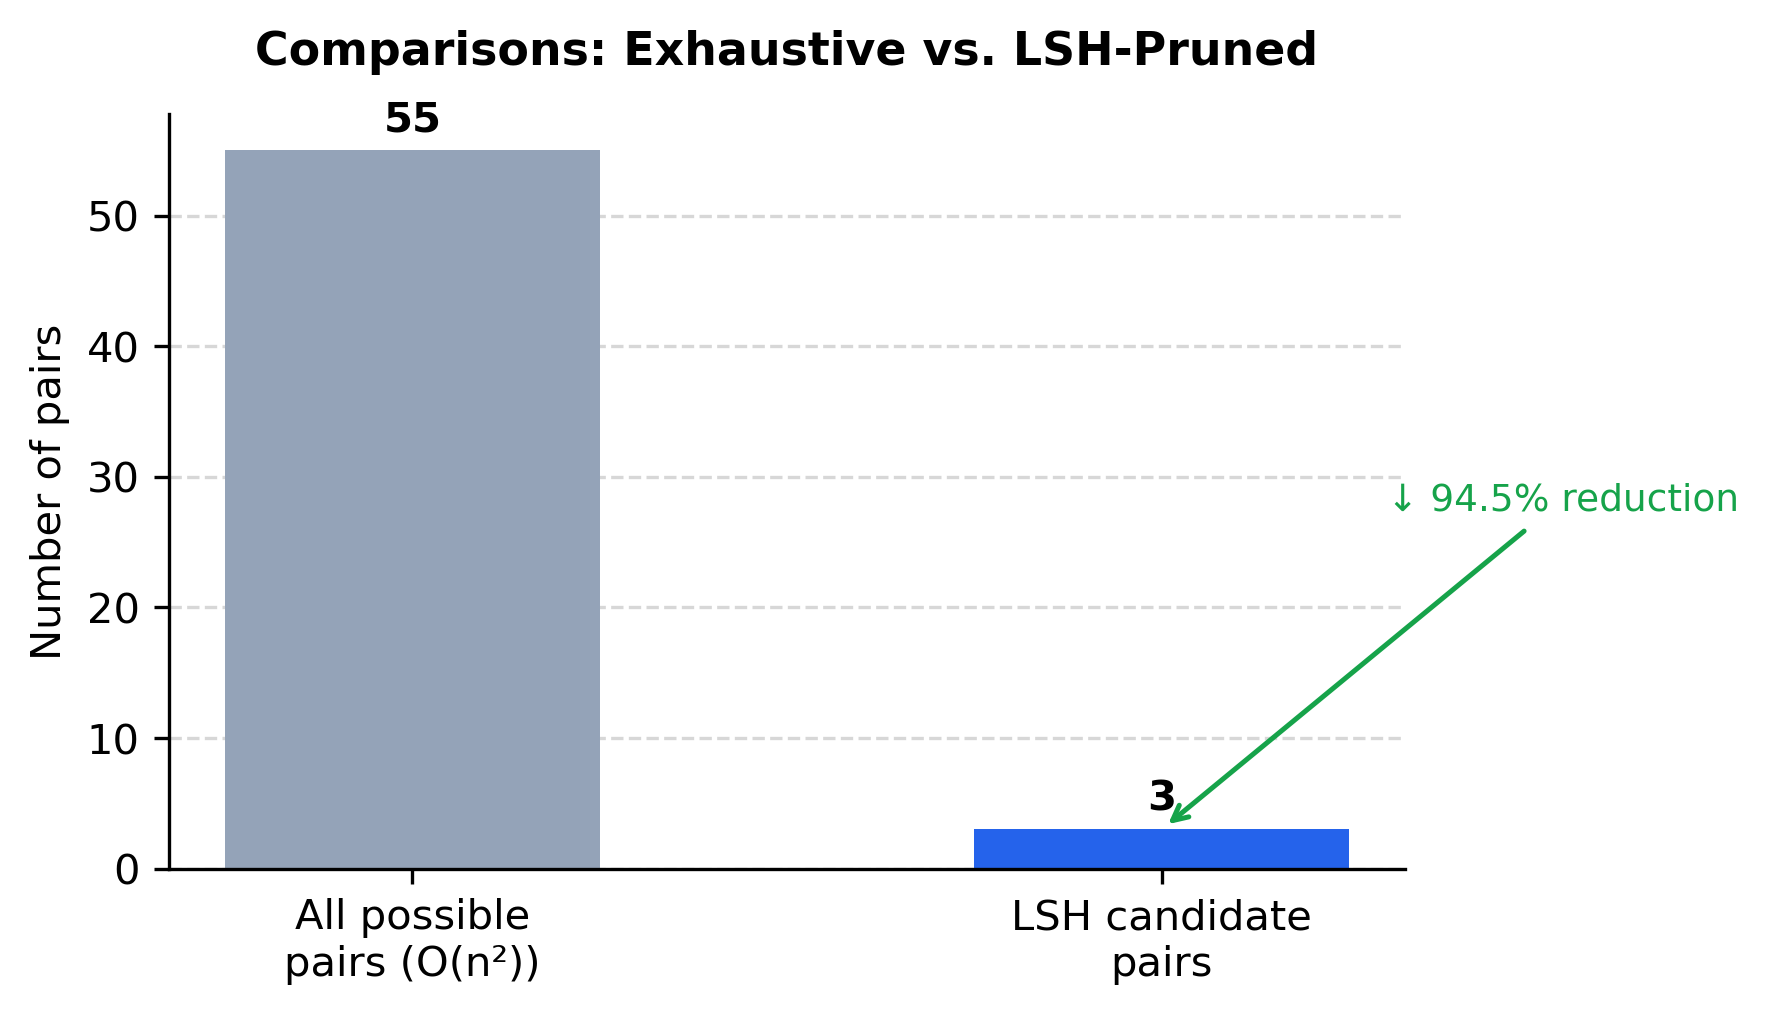
\includegraphics[width=0.62\textwidth]{figures/lsh_comparison.png}
		\caption{مقایسه‌ی کامل جفت‌به‌جفت (Exhaustive) در برابر جفت‌های کاندیدای \lr{LSH} که در عمل راستی‌آزمایی شدند روی پیکره‌ی نمونه.}
		\label{fig:comparisons-avoided}
	\end{figure}
	
	هر سه جفت کاندیدای نمایان‌شده، در واقع موارد تکراریِ واقعی بودند، و راستی‌آزمایی دقیق، امتیازهای شباهت آن‌ها را به‌طور کامل تأیید کرد (جدول~\ref{tab:candidates}) — این داده‌ها عیناً از فایل \lr{\texttt{outputs/candidates.csv}} استخراج و بازتولید شده‌اند.
	
\begin{table}[H]
	\centering
	\caption{Content of the \texttt{outputs/candidates.csv} file (with threshold = $0.25$).}
	\label{tab:candidates}
	\begin{tabular}{@{}llrr@{}}
		\toprule
		Doc A & Doc B & Exact Jaccard & MinHash Estimate \\
		\midrule
		doc\_$01$.txt & doc\_$03$.txt & $1.0000$ & $1.0000$ \\
		doc\_$01$.txt & doc\_$11$.txt & $0.4835$ & $0.5312$ \\
		doc\_$03$.txt & doc\_$11$.txt & $0.4835$ & $0.5312$ \\
		\bottomrule
	\end{tabular}
\end{table}


	
	به‌طور خاص توجه داشته باشید که جفت‌اسناد با بازنویسی سنگین (یعنی \lr{\texttt{doc\_01.txt}}/\lr{\texttt{doc\_02.txt}} و \lr{\texttt{doc\_04.txt}}/\lr{\texttt{doc\_05.txt}}) در این جدول حضور \emph{ندارند} — دلیل این پدیده در بخش ارزیابی خطاها تحلیل شده است.
	
	\subsection{مثال‌هایی از مقایسه دو سند}
	
	اجرای مستقیم فرمان \lr{\texttt{plagiarism\_engine.cli compare}} روی جفت‌های منفرد، رفتار هر دو موتور را در دو سر طیف دشواری به تصویر می‌کشد (جدول~\ref{tab:compare-examples}).
	
\begin{table}[H]
	\centering
	\caption{Output of the \texttt{compare} command for four sample document pairs.}
	\label{tab:compare-examples}
	\resizebox{\textwidth}{!}{%
		\begin{tabular}{@{}lrrrr@{}}
			\toprule
			Document Pair & Exact Jaccard & MinHash Estimate & LSH Candidate & SimHash Similarity \\
			\midrule
			doc\_$01$ / doc\_$03$ (verbatim copy) & $1.0000$ & $1.0000$ & Yes & $1.0000$ \\
			doc\_$01$ / doc\_$11$ (minor edit) & $0.4835$ & $0.5312$ & Yes & $0.8125$ \\
			doc\_$01$ / doc\_$02$ (heavy rewrite) & $0.0238$ & $0.0312$ & No & $0.6875$ \\
			doc\_$04$ / doc\_$05$ (heavy rewrite) & $0.0183$ & $0.0156$ & No & $0.6406$ \\
			\bottomrule
		\end{tabular}%
	}
\end{table}


	
	در تمامی حالات، تخمین \lr{MinHash} بسیار نزدیک به شباهت دقیق جاکارد عمل می‌کند (میانگین خطای مطلق برابر با $0.0021$ در تمامی ۵۵ جفت پیکره که در فایل \lr{\texttt{notebooks/exploration.ipynb}} محاسبه شده است)، که این امر تأیید می‌کند برآوردگر دقیقاً مطابق با پیش‌بینی تئوری رفتار می‌کند. در مقابل، شباهت همینگ در الگوریتم \lr{SimHash} تحت شرایط بازنویسی سنگین، رفتار بسیار ملایم‌تر و منعطف‌تری دارد (افت به بازه‌ی ۰٫۶۴ تا ۰٫۶۹ به‌جای فروپاشی به نزدیک صفر)؛ چرا که این روش روی یک \emph{کیسه‌ی کلماتِ وزن‌دار} کار می‌کند و نه روی $k$-گرام‌های پیوسته و دقیق؛ بنابراین تا زمانی که واژگان زیربنایی تا حد زیادی حفظ شده باشند، این الگوریتم در برابر تغییر ترتیب جملات و تغییرات نگارشی محلی مقاوم باقی می‌ماند (\lr{Graceful Degradation}).
	
	\begin{figure}[H]
		\centering
		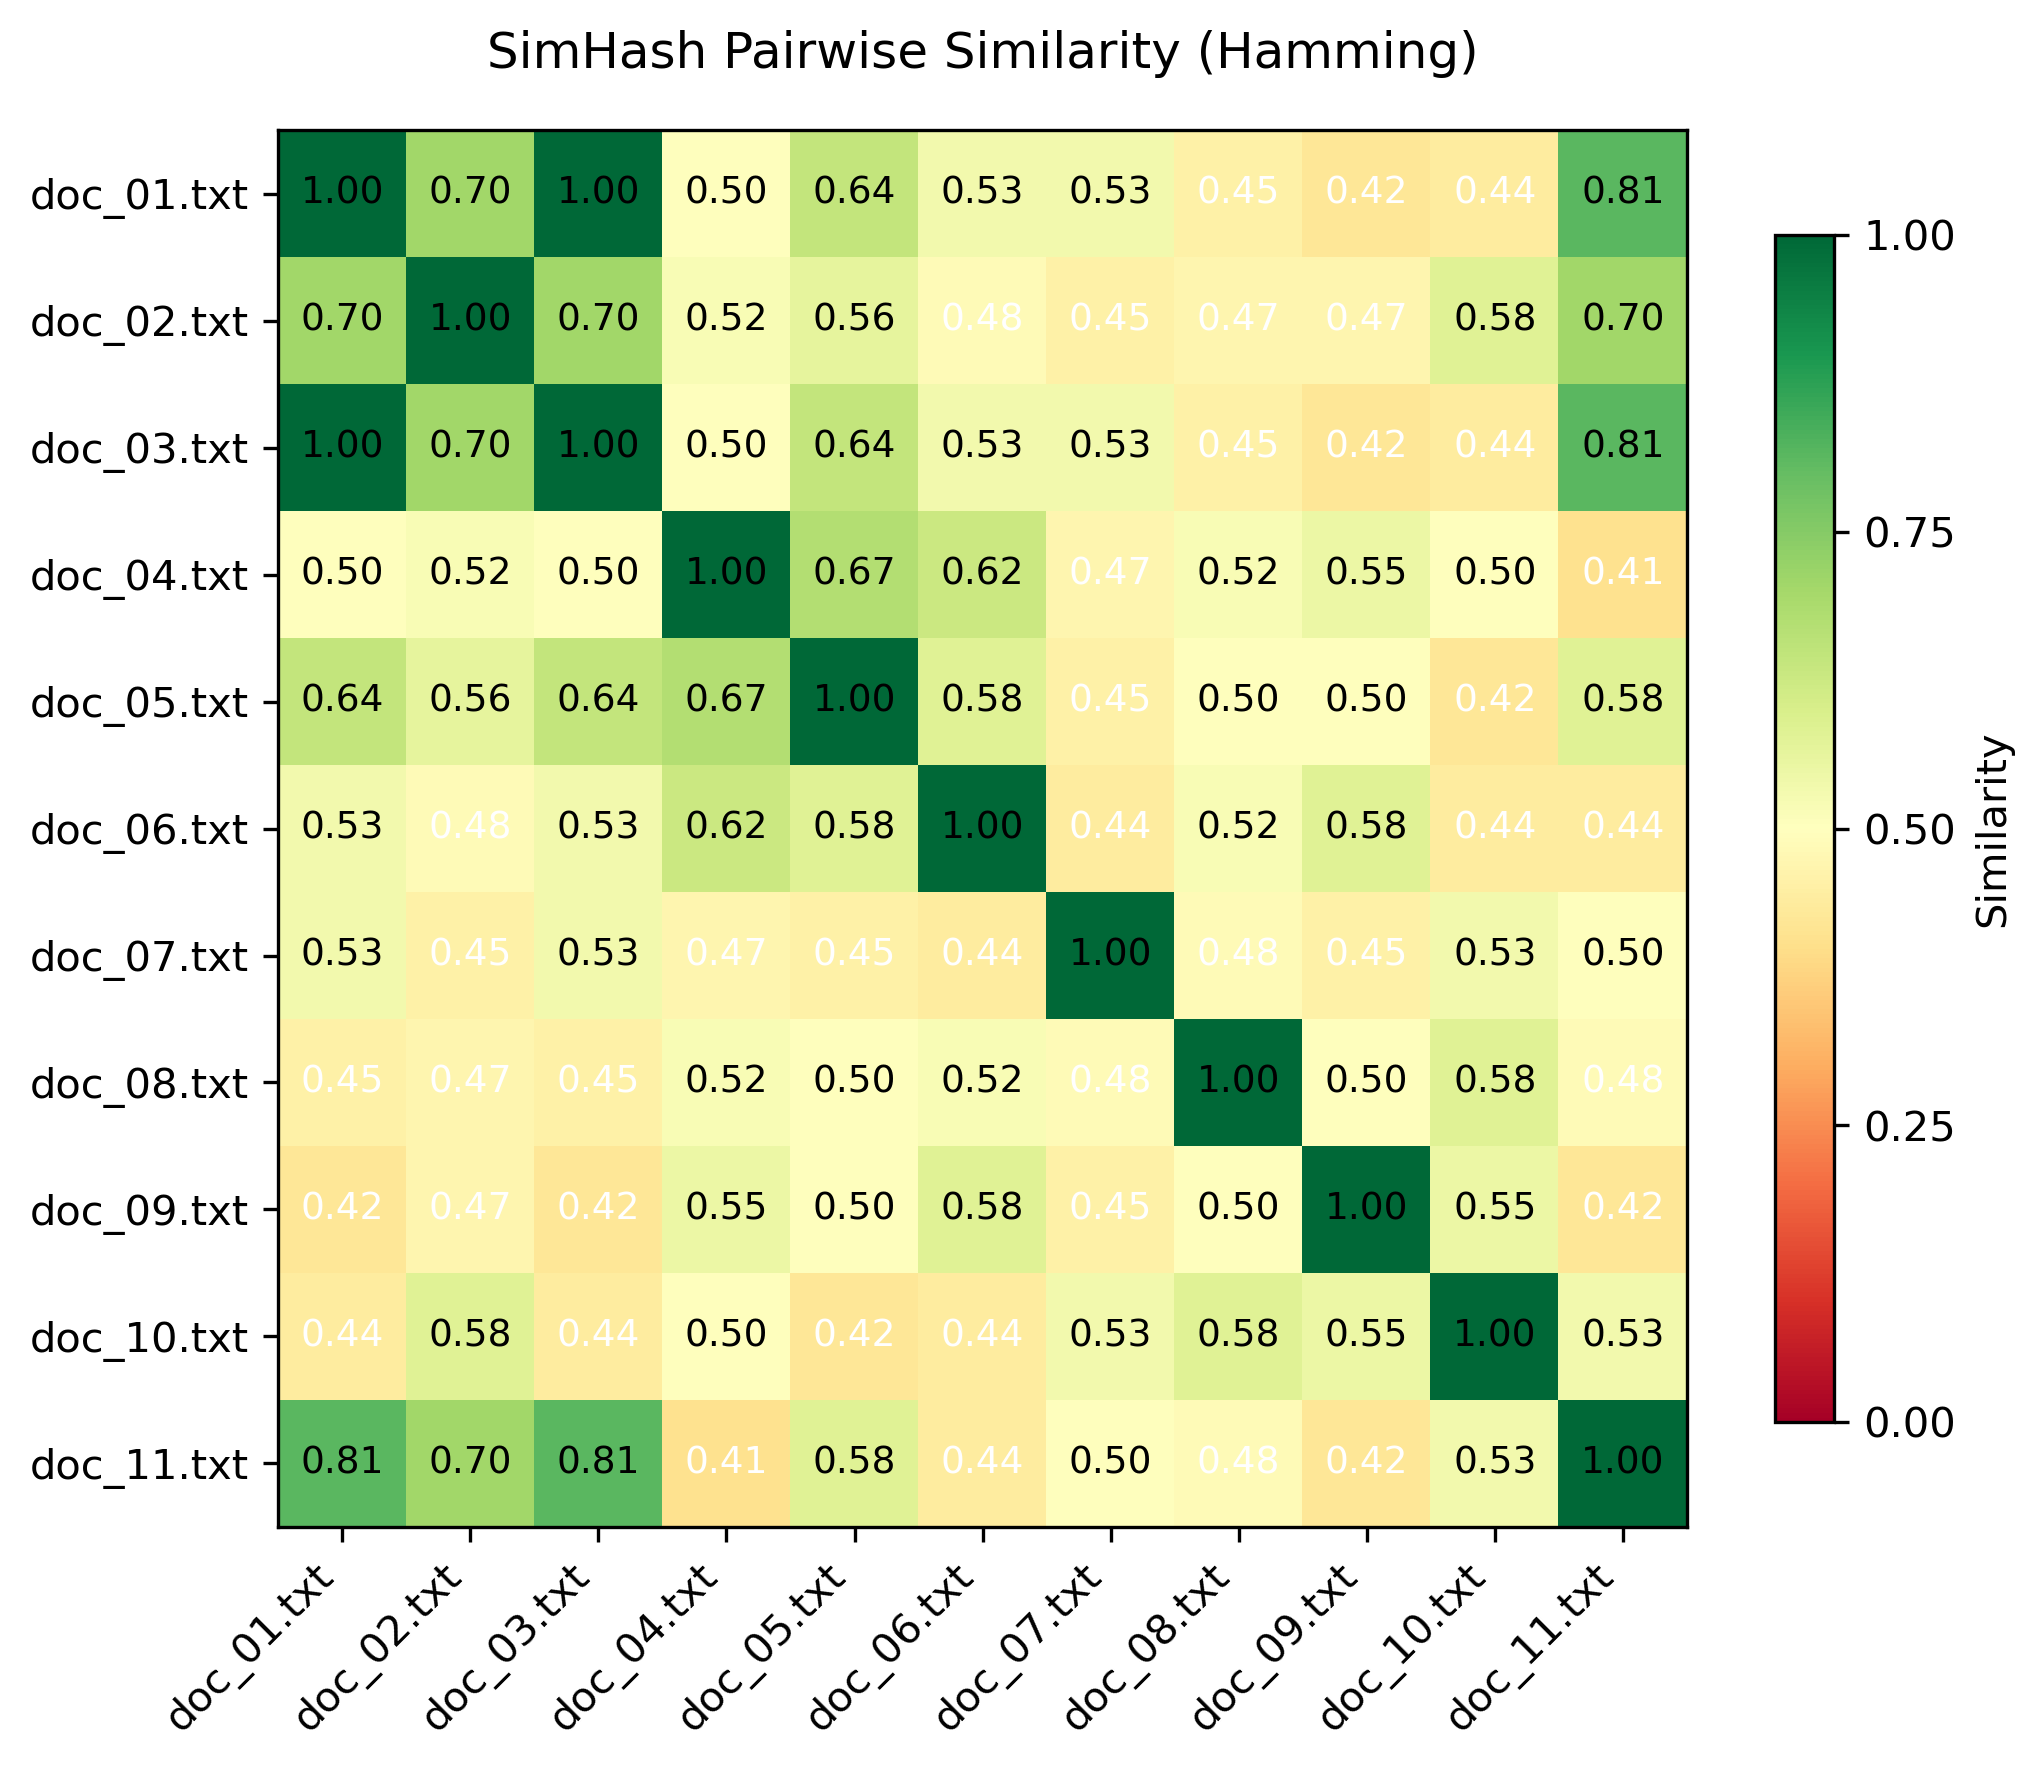
\includegraphics[width=0.85\textwidth]{figures/simhash_similarity_heatmap.png}
		\caption{نقشه‌ی حرارتی (Heatmap) شباهت همینگ در روش \lr{TF-IDF Weighted SimHash} برای تمام جفت‌های پیکره‌ی نمونه‌ی ۱۱ سندی (محاسبه‌ی \lr{IDF} روی کل پیکره انجام شده است).}
		\label{fig:simhash-heatmap}
	\end{figure}
	
	\subsection{نتایج روی مجموعه‌داده‌ی جفت‌ها: دقت، فراخوانی، \lr{F1} و زمان‌بندی}
	
	جدول~\ref{tab:pairs-metrics} نتایج مندرج در فایل \lr{\texttt{outputs/metrics.csv}} را بازتولید می‌کند که با اجرای فرمان زیر:
	
\begin{latin}
	\begin{lstlisting}
		python -m plagiarism_engine.cli pairs \
		--pairs data/raw/quora/sample_pairs.csv \
		--text-col-a question1 --text-col-b question2 --label-col is_duplicate \
		--shingle-size 1 --minhash-threshold 0.13 --simhash-threshold 0.46 \
		--output outputs/metrics.csv
	\end{lstlisting}
\end{latin}

	و با استفاده از پارامترهای تنظیم‌شده در بخش~\ref{sec:params} (اندازه شینگل $k=1$ برای متن‌های با طول پرسش، و آستانه‌های انتخاب‌شده از جاروب آستانه در جدول~\ref{tab:threshold-sweep}) به‌دست آمده است.
	
\begin{table}[H]
	\centering
	\caption{Precision, Recall, F1 score, and result counts on the $60$-pair synthetic dataset. Exact reproduction from the \texttt{outputs/metrics.csv} file.}
	\label{tab:pairs-metrics}
	\begin{tabular}{@{}lrrrr@{}}
		\toprule
		Method & Precision & Recall & F1 Score & TP/FP/FN/TN \\
		\midrule
		MinHash+LSH & $0.7297$ & $0.9000$ & $0.8060$ & $27/10/3/20$ \\
		TF-IDF SimHash & $0.5556$ & $1.0000$ & $0.7143$ & $30/24/0/6$ \\
		\bottomrule
	\end{tabular}
\end{table}


	
	\begin{figure}[H]
		\centering
		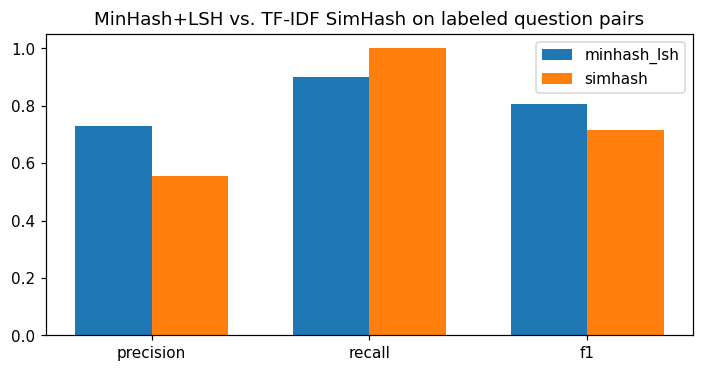
\includegraphics[width=0.62\textwidth]{figures/method_comparison_pairs.png}
		\caption{مقایسه دقت، فراخوانی و امتیاز \lr{F1} برای هر دو موتور روی مجموعه‌داده‌ی مصنوعی جفت‌های برچسب‌دار.}
		\label{fig:method-comparison}
	\end{figure}
	
	در آستانه‌های کالیبره‌شده‌ی مربوط به هر روش، خط لوله‌ی \lr{MinHash+LSH} به دقت و امتیاز \lr{F1} بالاتری دست می‌یابد، در حالی که \lr{SimHash} فراخوانیِ کامل (۱۰۰٪) را به قیمت تولید موارد مثبت کاذبِ (False Positives) بسیار بیشتر به دست می‌آورد — این الگوریتم ۲۴ مورد از ۳۰ منفیِ واقعی را به‌اشتباه به‌عنوان تکراری علامت‌گذاری می‌کند. همچنین \lr{SimHash} در این آزمایش تقریباً ۵٫۶ برابر سریع‌تر به ازای هر جفت عمل می‌کند؛ زیرا مقایسه‌ی فاصله‌ی همینگ میان دو عدد ۶۴-بیتی از مرتبه‌ی زمانی $O(1)$ است، در حالی که مقایسه‌ی \lr{MinHash} از مرتبه‌ی $O(\text{num\_perm})$ (در اینجا ۱۲۸ مقایسه به ازای هر جفت) به علاوه‌ی هزینه‌ی ساخت هر امضا از روی مجموعه‌ی شینگل‌های آن است. \emph{این زمان‌بندی‌های مطلق صرفاً جنبه‌ی نمایشی دارند} و روی یک مجموعه‌داده‌ی ۶۰ سطری در یک سیستم اشتراکی اندازه‌گیری شده‌اند؛ برتریِ کیفیِ مورد انتظار (کم‌هزینه‌تر بودن مقایسه‌ی اثرانگشت نسبت به مقایسه‌ی امضا به ازای هر جفت) به‌طور کلی برقرار است، اما هیچ‌یک از این اعداد نباید به‌عنوان یک بنچمارک در مقیاس صنعتی تلقی شوند. مزیت ساختاری بسیار بزرگ‌ترِ خط لوله‌ی \lr{MinHash+LSH} — یعنی اجتناب کامل از تعداد مقایسه‌های $O(n^2)$ در حجم کاریِ جست‌وجوی پیکره از طریق هرس کاندیداها توسط \lr{LSH} — در اجرای فرمان \lr{\texttt{pairs}} اصلاً مورد سنجش قرار نمی‌گیرد، زیرا این فرمان جفت‌های ازپیش‌تشکیل‌شده را ارزیابی می‌کند، نه اینکه کل یک پیکره را جست‌وجو کند؛ آن مزیت بزرگ به‌طور مستقل در بخش~\ref{sec:corpus-results} اثبات شد.
	
	\subsection{نتایج روی پیکره‌ی واقعی \lr{PAN-PC-11}}
	\label{sec:pan-pc11-results}
	
	مجموعه‌داده‌ی ۴٬۰۰۰ جفتیِ \lr{PAN-PC-11} که در بخش~\ref{sec:pan-pc11-dataset} ساخته شد، به سه روش مورد ارزیابی قرار گرفت تا اثرِ اندازه شینگل از اثرِ تنظیم و کالیبره‌سازیِ آستانه تفکیک شود:
	
\begin{table}[H]
	\centering
	\caption{Performance of MinHash+LSH and SimHash on the $4,000$-pair real-world evaluation dataset (PAN-PC-11), comparing two settings: fixed shingle size and threshold (suggested by project specifications) versus swept threshold and shingle.}
	\label{tab:pan-pc11-results}
	\begin{tabular}{@{}llrrrr@{}}
		\toprule
		Configuration & Method & Applied Threshold & Precision & Recall & F1 Score \\
		\midrule
		$k=3$, fixed ($0.5 / 0.85$) & MinHash+LSH   & $0.50$ & $1.0000$ & $0.0360$ & $0.0695$ \\
		$k=3$, fixed ($0.5 / 0.85$) & TF-IDF SimHash & $0.85$ & $1.0000$ & $0.0725$ & $0.1352$ \\
		$k=3$, with \texttt{--sweep}   & MinHash+LSH   & $0.00$ & $0.5000$ & $1.0000$ & $0.6667$ \\
		$k=3$, with \texttt{--sweep}   & TF-IDF SimHash & $0.58$ & $0.8389$ & $0.7445$ & $0.7889$ \\
		$k=1$, with \texttt{--sweep}   & MinHash+LSH   & $0.10$ & $0.9706$ & $0.8745$ & $0.9200$ \\
		$k=1$, with \texttt{--sweep}   & TF-IDF SimHash & $0.58$ & $0.8389$ & $0.7445$ & $0.7889$ \\
		\bottomrule
	\end{tabular}
\end{table}	
	\begin{figure}[H]
		\centering
		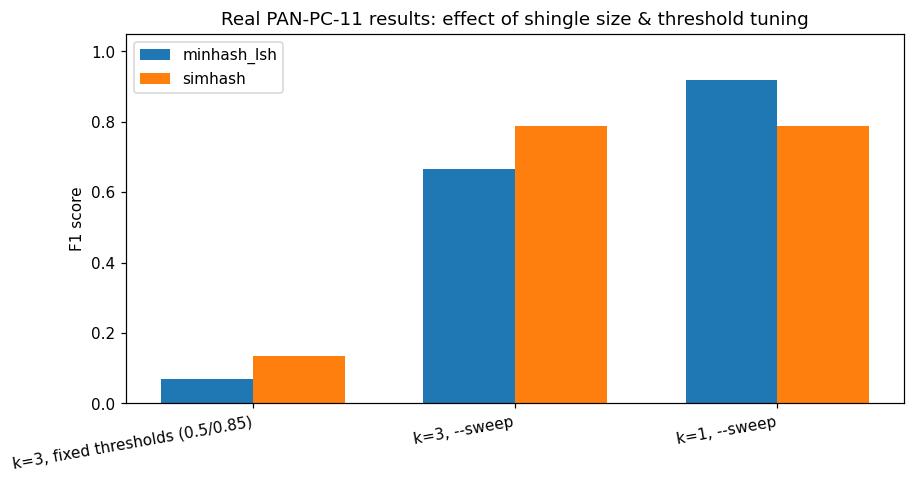
\includegraphics[width=0.75\textwidth]{figures/pan_pc11_f1_comparison.png}
		\caption{امتیاز \lr{F1} روی مجموعه‌ی ارزیابی واقعی \lr{PAN-PC-11} بر اساس اندازه شینگل و استراتژی انتخاب آستانه. ردیف مربوط به \lr{SimHash} در هر دو ستون $k=3$ و $k=1$ کاملاً یکسان است، چرا که پرچم \lr{\texttt{--shingle-size}} تنها خط لوله‌ی \lr{MinHash+LSH} را پارامتردهی می‌کند؛ عرضِ $n$-گرامِ توکن‌ها در الگوریتم \lr{SimHash} یک تنظیماتِ مستقل و (در حال حاضر) غیرقابل‌دسترسی از طریق خط فرمان است که به‌طور پیش‌فرض روی تک‌گرام (Unigram) قرار دارد (بخش محدودیت‌ها).}
		\label{fig:pan-pc11-f1}
	\end{figure}
	
	سه یافته‌ی تحلیلی و کلیدی از این نتایج استنتاج می‌شود:
	\textbf{اول:} آستانه‌های ثابتی که از پیکره‌ی دمو (با طول پاراگراف) به این پیکره منتقل شدند، به‌شدت برای این مجموعه‌داده کالیبره‌نشده هستند: هر دو روش به دقت کامل (۱۰۰٪) می‌رسند اما فراخوانی آن‌ها زیر ۷٫۵٪ است؛ این وضعیت، نشانه‌ی بارز و کلاسیکِ انتخاب یک آستانه‌ی بیش‌ازحد بالا است، نه نشانه‌ی خراب بودن معیار شباهت (به بخش انتخاب خودکار آستانه مراجعه کنید).
	\textbf{دوم:} صرفِ جاروب کردن آستانه (در حالی که همچنان $k=3$ است) برای \lr{MinHash+LSH} کافی نیست — آستانه‌ی بهینه‌ی بیشینه‌کننده‌ی \lr{F1} که پیدا می‌شود برابر با $0.00$ است؛ این یعنی فرایند جاروب کشف می‌کند که هیچ آستانه‌ای در $k=3$ برای روش \lr{MinHash+LSH} نمی‌تواند از خط پایه‌ی بدیهیِ «همه را تکراری پیش‌بینی کن» (که با توجه به نرخ ۵۰ درصدی کلاس مثبت، امتیاز $F_1=0.667$ دارد) بهتر عمل کند. این امر نشان می‌دهد که امتیازهای شباهت در $k=3$ اساساً هیچ سیگنالِ قابل‌استفاده‌ای در این مجموعه‌داده حمل نمی‌کنند. در مقابل، الگوریتم \lr{SimHash} حتی در حالت $k=3$ نیز یک نقطه‌ی عملیاتی منطقی و کارآمد را بازیابی می‌کند ($F_1=0.789$)؛ چرا که بازنمایی و اثرانگشت آن از همان ابتدا مستقل از ترتیب (Order-independent) است.
	\textbf{سوم:} کاهش اندازه شینگل به $k=1$، عملکرد بسیار قدرتمندی را برای خط لوله‌ی \lr{MinHash+LSH} بازیابی می‌کند ($F_1=0.920$، که بهترین نتیجه در میان تمام پیکربندی‌های این گزارش است)، که این موضوع مکانیزم تحلیلی شرح‌داده‌شده در بخش~\ref{sec:shingle-size-pan} را تأیید می‌کند: مبهم‌سازی‌های پراکنده در پیکره‌ی \lr{PAN-PC-11} آسیب به‌مراتب بیشتری به $k$-گرام‌های پیوسته وارد می‌کنند تا به هم‌پوشانی ساده‌ی کلمات. نکته‌ی بسیار حائز اهمیت این است که رتبه‌بندیِ نسبیِ این دو روش میان این مجموعه‌داده و مجموعه‌داده‌ی مصنوعی جفت‌پرسش در جدول~\ref{tab:pairs-metrics} \emph{کاملاً معکوس} می‌شود (در آنجا فراخوانی \lr{SimHash} برتری داشت؛ اما در اینجا امتیاز \lr{F1} در روش \lr{MinHash+LSH} مسلط است) — بخش ارزیابی خطاها به‌طور مفصل توضیح می‌دهد که چرا طول سند و سبک مبهم‌سازی عامل اصلی این پدیده هستند، نه اینکه یکی از روش‌ها به‌طور مطلق و ذاتی «بهتر» از دیگری باشد.
	
	
	
	% =========================================================================
	\section{تحلیل خطا}
	\label{sec:error-analysis}
	% =========================================================================
	
	این بخش به بررسی نمونه‌های مشخصی از دسته‌بندی‌های اشتباه می‌پردازد که مستقیماً از آزمایش‌های فوق استخراج شده‌اند، و نشان می‌دهد که این موارد درباره‌ی حالت‌های شکست (Failure Modes) هر روش چه حقایقی را آشکار می‌سازند.
	
	\subsection{ترکیب \lr{MinHash+LSH}: منفی‌های کاذب در بازنویسی‌های سنگین}
	\label{sec:error-analysis-heavy}
	
	هر سه مورد منفی کاذبِ \lr{MinHash+LSH} در آستانه‌ی تنظیم‌شده ($k=1$، آستانه $0.13$)، جفت‌های \lr{heavy\_duplicate} (تکراری‌های سنگین) هستند -- یعنی جفت‌های تکراری واقعی که تقریباً با واژگانی کاملاً متفاوت بیان شده‌اند:
	
	\begin{itemize}
		\item \emph{«فواید مدیتیشن منظم چیست؟»} در برابر \emph{«تمرین منظم مدیتیشن چگونه به یک فرد کمک می‌کند؟»} (شباهت $0.102$، زیر آستانه)
		\item \emph{«چگونه سگ مضطرب خود را در طول طوفان رعد و برق آرام کنم؟»} در برابر \emph{«وقتی سگم از رعد و برق می‌ترسد برای تسکین او چه کار کنم؟»} (شباهت $0.078$)
		\item \emph{«تفاوت بین ویروس و باکتری چیست؟»} در برابر \emph{«ویروس‌ها چه تفاوتی با باکتری‌ها دارند؟»} (شباهت $0.094$)
	\end{itemize}
	
	این همان نقطه ضعف ساختاری و مورد انتظار شباهت ژاکارد (\lr{Jaccard}) مبتنی بر شینگل (\lr{shingle}) است: این روش معیاری از هم‌پوشانی \emph{واژگانی (Lexical)} است، نه هم‌ارزی معنایی. هنگامی که در یک بازنویسی، اکثر کلمات محتوایی با مترادف‌ها جایگزین می‌شوند (تسکین دادن $\leftrightarrow$ آرام کردن، ترس از رعد و برق $\leftrightarrow$ در طول طوفان)، مجموعه‌های شینگل می‌توانند تقریباً مجزا از هم شوند، حتی با وجود اینکه یک خواننده‌ی انسانی بلافاصله این سوالات را به عنوان موارد تکراری تشخیص می‌دهد. همین پدیده توضیح می‌دهد که چرا جفت اسناد با بازنویسی سنگین در پیکره‌ی نمونه (\lr{\texttt{doc\_01.txt}}/\lr{\texttt{doc\_02.txt}} و \lr{\texttt{doc\_04.txt}}/\lr{\texttt{doc\_05.txt}}) علیرغم اینکه بازنویسی‌های واقعیِ یکدیگر بودند، به عنوان کاندیداهای \lr{LSH} در جدول~\ref{tab:candidates} ظاهر نشدند.
	
	\subsection{ترکیب \lr{MinHash+LSH} و \lr{SimHash}: مثبت‌های کاذب در منفی‌های دشوار}
	\label{sec:error-analysis-hard}
	
	هر ۶ جفت منفیِ دشوار (\lr{hard-negative}) (الگوی یکسان، تنها با تغییر یک کلمه محتوایی) توسط \emph{هر دو} روش به اشتباه به عنوان تکراری طبقه‌بندی شدند، برای مثال:
	
	\begin{itemize}
		\item \emph{«بهترین راه برای پختن برنج روی اجاق گاز چیست؟»} در برابر \emph{«بهترین راه برای پختن کینوا روی اجاق گاز چیست؟»} -- شباهت \lr{MinHash+LSH} برابر $0.695$؛ شباهت \lr{SimHash} برابر $0.688$.
		\item \emph{«چگونه در بزرگسالی نواختن پیانو را یاد بگیرم؟»} در برابر \emph{«چگونه در بزرگسالی شطرنج بازی کردن را یاد بگیرم؟»} -- شباهت \lr{MinHash+LSH} برابر $0.734$؛ شباهت \lr{SimHash} برابر $0.672$.
	\end{itemize}
	
	این جفت‌ها در ۸ کلمه از ۹ کلمه (یا بیشتر) کاملاً یکسان هستند و فقط در یک کلمه‌ی محتوایی که کل معنی سوال را تغییر می‌دهد متفاوتند. هیچ روش کاملاً واژگانی -- چه مبتنی بر هم‌پوشانی مجموعه (\lr{MinHash}) و چه مبتنی بر کیسه کلمات وزن‌دار (\lr{SimHash}) -- نمی‌تواند «برنج» را از «کینوا» به عنوان \emph{موضوعات متفاوت} تشخیص دهد؛ بلکه هر دو صرفاً ابعاد متمایزی در فضای توکن هستند و بدون توجه به اینکه از نظر معنایی چقدر متفاوتند، به یک اندازه در میزان اختلاف نقش دارند. تشخیص این دسته از خطاها نیازمند بازنمایی‌ای است که \emph{معنای} کلمه را درک کند (مانند تعبیه‌های کلمه یا جمله - \lr{embeddings})، که صراحتاً خارج از محدوده این پروژه است.
	
	\subsection{نمایه خطای نامتقارن \lr{SimHash}}
	
	موارد مثبت کاذب \lr{SimHash} (۲۴ مورد از ۳۰ منفی واقعی، شامل بسیاری از جفت‌های \lr{easy\_negative} با موضوعات کاملاً بی‌ربط، مثلاً \emph{«تفاوت بین یادگیری ماشین و یادگیری عمیق چیست؟»} در برابر \emph{«تفاوت بین ویروس و باکتری چیست؟»}، شباهت $0.734$) پرشمارتر هستند و به منفی‌های دشوار محدود نمی‌شوند. ما این مسئله را به یک انتخاب طراحی خاص در خط لوله‌ی ارزیابی \lr{\texttt{pairs}} نسبت می‌دهیم: برای مستقل نگه‌داشتن ارزیابی هر جفت، فایل \lr{\texttt{evaluation.py}} آمارهای \lr{IDF} را \emph{فقط روی دو سند موجود در همان جفت} (ببینید \lr{\texttt{run\_simhash\_pipeline}}) برازش (Fit) می‌کند، نه روی کل مجموعه‌داده. با وجود تنها دو سند، فرکانس سند (\lr{Document Frequency}) یک عبارت فقط می‌تواند مقادیر ۱ یا ۲ را بگیرد -- تقریباً هیچ مفهوم مفیدی از کمیابی در سطح کل پیکره برای بهره‌برداری وجود ندارد، بنابراین وزن‌های به‌دست‌آمده تقریباً یکنواخت می‌شوند و عملکرد \lr{SimHash} به سمت یک مقایسه‌ی کیسه کلماتِ بدون وزن تنزل می‌یابد. در نتیجه، هر دو سوال انگلیسی با طول مشابه و ساختار جمله‌ی مشابه (مانند «چیست...»، «چگونه...») صرفاً به دلیل کلمات تابعی (Function Words) و توکن‌های ساختاری مشترک، به یک شباهت پایه‌ی همینگ (\lr{Hamming}) در حد متوسط دست می‌یابند، که آستانه $0.46$ -- که برای به حداکثر رساندن $F_1$ در کل مجموعه‌داده تنظیم شده است -- آن‌قدر سخت‌گیرانه نیست که بتواند آن‌ها را در هر حالتی فیلتر کند. این یک هزینه‌ی مستقیم و قابل‌اندازه‌گیری از طراحی ارزیابیِ جفت‌به‌جفت است و در شکل~\ref{fig:simhash-heatmap} در نقطه مقابل قابل مشاهده است؛ جایی که \lr{SimHash} یک بار روی کل پیکره‌ی نمونه ۱۱-سندی برازش شده است: در آنجا، جفت اسناد با موضوعات نامرتبط (مانند پاراگراف آشپزی در برابر پاراگراف اکتشاف مریخ) به طور مشهودی شباهت پایین‌تری نسبت به جفت‌های مرتبط نشان می‌دهند، زیرا \lr{IDF} در سطح پیکره اسناد کافی برای کاهش وزن کلمات رایج عمومی در اختیار دارد. \textbf{توصیه}: برای استقرار در مقیاس پیکره، چنانچه یک مجموعه‌داده‌ی برچسب‌دار از جفت‌ها از یک پیکره‌ی زیربنایی منسجم استخراج شده است، \lr{IDF} مربوط به \lr{SimHash} را یک بار روی کل پیکره (همان‌طور که دستور \lr{\texttt{corpus}} می‌تواند انجام دهد و در دفترچه یادداشتِ اکتشافی انجام شده است) برازش کنید، نه به‌صورت جفت‌به‌جفت.
	
	\subsection{یک هشدار روش‌شناختی درباره هم‌پوشانی کلمات پرسشی}
	
	یک اثر ثانویه و کوچکتر: با شینگل‌های $k=1$ (یونی‌گرم)، کلمات پرسشی رایج مانند \emph{``how''}, \emph{``do''}, \emph{``what''}, و \emph{``is''} در لیست حداقل کلمات توقف (Stop Words) ما (بخش~۲) قرار \textbf{نمی‌گیرند}، زیرا آن لیست به جای کلمات خاص پرسشی، کلمات تابعی بسته را هدف قرار می‌دهد. بنابراین، دو سوال نامرتبط که هر دو با «چگونه من...» شروع می‌شوند، به دلیل کلمات الگوی جمله، مقداری هم‌پوشانی پایه‌ی یونی‌گرمی دارند که در چندین مثبت کاذبِ منفی-آسانِ \lr{MinHash} نقش دارد (مثلاً \emph{«چگونه یک لپ‌تاپ کند را تعمیر کنم؟»} در برابر \emph{«گیاهان چگونه غذای خود را می‌سازند؟»}، شباهت $0.172$، درست بالای آستانه $0.13$). یک لیست کلمات توقفِ دامنه-خاص برای پیکره‌های پرسش‌وپاسخ (با گسترش لیست پایه با کلمات پرسشی) احتمالاً این دسته از خطاها را کاهش می‌دهد؛ ما در اینجا این کار را انجام ندادیم تا لیست کلمات توقف را به عنوان یک پیاده‌سازی وفادار و حداقلی از نیازمندی‌های صریح مشخصات پروژه (کلمات ``and'', ``is'', ``the'', ``or'' و معادل‌های فارسی) نگه داریم و آن را روی یک مجموعه‌داده‌ی خاص بیش‌برازش (\lr{Overfit}) نکنیم.
	
	\subsection{مجموعه‌داده‌ی واقعی \lr{PAN-PC-11}: فروپاشی فراخوانی به دلیل مبهم‌سازی، و چراییِ وابسته‌بودن راه‌حل به مجموعه‌داده}
	\label{sec:error-analysis-pan}
	
	بخش~\ref{sec:pan-pc11-results} نشان داد که با استفاده از آستانه‌های ثابت، فراخوانیِ \lr{MinHash+LSH} در $k=3$ به $3.6\%$ سقوط کرد. به بیان دقیق‌تر: با میانگین طول قطعه در حدود چند هزار کاراکتر، یک شینگل ۳-کلمه‌ای تنها زمانی زنده می‌ماند که هر سه کلمه‌ی متوالی بدون ویرایش باقی بمانند. استراتژی مبهم‌سازی (Obfuscation) «مصنوعی» \lr{PAN-PC-11} (طبق مستندات خود پیکره) جایگزینی‌هایی را اعمال می‌کند که به جای تمرکز در یک نقطه، در سراسر متن توزیع شده‌اند. بنابراین، حتی یک نرخ متوسط جایگزینی کلمه می‌تواند باعث شود که تقریباً هیچ ۳-گرمی (\lr{3-gram}) به‌صورت کامل دست‌نخورده باقی نماند -- مقدار ژاکارد دقیق برای ۳-شینگل می‌تواند به شکل موجهی برای جفتی که انسان بلافاصله آن را همان متن (اما ویرایش‌شده) تشخیص می‌دهد، به زیر $0.05$ برسد. این دقیقاً همان حالت شکستِ اساسی است که برای بازنویسی‌های سنگین در بخش~\ref{sec:error-analysis-heavy} مستند شده است، با این تفاوت که بسیار شدیدتر است زیرا مبهم‌سازی \lr{PAN-PC-11} متراکم‌تر بوده و قطعات طولانی‌تر هستند (فرصت‌های بیشتری برای افتادن یک کلمه جایگزین‌شده در داخل هر شینگل وجود دارد). شینگل‌بندی یونی‌گرمی از این مشکل عبور می‌کند زیرا یک کلمه‌ی جایگزین شده تنها \emph{یک} عنصر را از مجموعه‌ای متشکل از صدها یا هزاران عضو حذف می‌کند، نه اینکه زنجیره‌ای از ۳-گرم‌های هم‌پوشان را نابود کند.
	
	\textbf{چرا راه‌حل (استفاده از $k$ کوچکتر) به جای اینکه جهان‌شمول باشد، به مجموعه‌داده وابسته است:} کاهش $k$ حساسیت به ترتیب کلمات و ساختار عبارت را از بین می‌برد. برای پیکره‌ای که در آن اسنادِ تقریباً تکراری غالباً کپی‌های کلمه‌به‌کلمه یا با ویرایش کم هستند (مانند پیکره‌ی نمونه‌ی پاراگراف‌محور در بخش~\ref{sec:corpus-results})، $k=3$ جفت‌های نامربوط را به درستی رد می‌کند دقیقاً به این دلیل که نیازمند تطابق پیوسته است؛ تغییر آن به $k=1$ در آنجا باعث افزایش نرخ مثبت‌های کاذب در میان اسنادِ با موضوعِ مشابه-اما-متمایز می‌شود (همان سازوکاری که به عنوان حالت شکستِ «منفیِ دشوار» در بخش~\ref{sec:error-analysis-hard} برای جفت سوالات مستند شد). بنابراین، اندازه مناسب شینگل تابعی از \emph{نحوه} تفاوت اسنادِ تقریباً تکراریِ یک پیکره نسبت به منبع آنهاست -- ویرایش‌های متمرکز نیازمند $k$ بزرگتر هستند؛ ویرایش‌های پراکنده نیازمند $k$ کوچکتر -- به همین دلیل است که این گزارش با آن به عنوان یک فراپارامتر (Hyperparameter) قابل تنظیم رفتار می‌کند (بخش~\ref{sec:shingle-size-pan}) نه اینکه یک مقدار ثابت «صحیح» را پیشنهاد دهد.
	
	\textbf{چرا رتبه‌بندی \lr{SimHash} و \lr{MinHash+LSH} در میان مجموعه‌داده‌ها جابجا می‌شود:} در جفت سوالات ترکیبی کوتاه (جدول~\ref{tab:pairs-metrics})، وزن‌دهی \lr{TF-IDF} در \lr{SimHash} سیگنال قابل استفاده‌ی بیشتری از متون بسیار کوتاه نسبت به ژاکاردِ $k$-گرم استخراج کرد؛ در قطعات متنیِ بلند \lr{PAN-PC-11} (جدول~\ref{tab:pan-pc11-results})، \lr{MinHash+LSH} با یونی‌گرم، \lr{SimHash} را شکست می‌دهد. ما این موضوع را به معنای برتری مطلق هیچ‌کدام از روش‌ها نمی‌دانیم -- هر دو روش در هسته‌ی خود معیارهای واژگانی از نوع کیسه‌ای (\lr{Bag-of-something}) هستند، و اینکه کدام یک پیروز می‌شود به طول سند و الگوی فضایی ویرایش‌ها در آن پیکره‌ی خاص بستگی دارد. این دقیقاً استدلالی در حمایت از پیاده‌سازی و مقایسه \emph{دو} روش مستقل است، به جای اینکه همان‌طور که در مشخصات پروژه نیز خواسته شده، تنها به یکی بسنده کنیم.
	
	\textbf{تعامل با محدودیت عدم‌تطابق طول (بخش~\ref{sec:pan-pc11-dataset}):} از آنجایی که قطعاتِ مثبت می‌توانند بسیار طولانی‌تر از بخش‌های کوتاه شده‌ی منفی باشند، بخشی از تفکیک‌پذیری ظاهری در جدول~\ref{tab:pan-pc11-results} ممکن است صرفاً ناشی از خود طول باشد تا مقاومت در برابر مبهم‌سازی. این مسئله نتیجه‌گیری \emph{نسبی} مبنی بر اینکه $k=1$ سیگنال بیشتری را نسبت به $k=3$ تحت مبهم‌سازیِ پراکنده بازیابی می‌کند، تغییر نمی‌دهد (هر دو پیکربندی در این مجموعه‌داده‌ی یکسان و با عدم‌تطابقِ طول برابر ارزیابی شده‌اند)، اما به این معنی است که مقدار مطلق $F_1=0.920$ نباید به عنوان یک اندازه‌گیری تمیز و کنترل‌شده-از-نظر-طول برای عملکرد کشف سرقت ادبی در دنیای واقعی ذکر شود.
	% =========================================================================
	\section{نتیجه‌گیری}
	% =========================================================================
	
	ما از پایه، هم یک خط لوله \lr{Shingling + MinHash + LSH} و هم یک خط لوله \lr{SimHash} وزن‌دار با \lr{TF-IDF} را برای کشف تکراری‌های معنایی و سرقت‌های ادبی پیاده‌سازی کردیم، هر دو را از طریق یک \lr{CLI} با سه دستور (\lr{\texttt{compare}}, \lr{\texttt{corpus}}, \lr{\texttt{pairs}}) در دسترس قرار دادیم و آن‌ها را بر روی سه مجموعه‌داده ارزیابی کردیم: یک پیکره دست‌چین شده از اسناد، یک مجموعه‌داده ترکیبی برچسب‌دار از جفت-سوالات و پیکره واقعی سرقت ادبی \lr{PAN-PC-11} شامل $22{,}186$ جفت. هرس کاندیداهای \lr{LSH} از انجام $94.55\%$ مقایسه‌های دوبه‌دو در پیکره نمونه جلوگیری کرد در حالی که هیچ یک از موارد شبه‌تکراریِ واقعیِ بالای آستانه را از دست نداد، و تخمین ژاکاردِ \lr{MinHash} به خوبی ژاکارد دقیق را دنبال کرد (میانگین خطای مطلق $0.0021$). در ارزیابی جفت-سوالات ترکیبی، \lr{MinHash+LSH} در یک نقطه‌ی عملیاتی تنظیم‌شده به دقت (Precision) و \lr{F1} بالاتری ($0.730$ / $0.806$) رسید، در حالی که \lr{SimHash} به فراخوانی (Recall) کامل ($1.000$) اما با دقت پایین‌تر ($0.556$) دست یافت. در پیکره واقعی \lr{PAN-PC-11}، شینگل $k=3$ که در مشخصات پروژه توصیه‌شده بود در ترکیب با آستانه‌های تنظیم‌نشده باعث فروپاشی فراخوانیِ \lr{MinHash+LSH} به $3.6\%$ علیرغم دقت کامل شد -- که این یک شکست در کالیبراسیون آستانه بود، نه یک شکست الگوریتمی -- این مسئله انگیزه اضافه کردن قابلیت انتخاب خودکار آستانه (\lr{\texttt{--sweep}}) به ابزار را ایجاد کرد؛ با کاهش اندازه شینگل به $k=1$ برای مقابله با مبهم‌سازی پراکنده در سطح کلماتِ \lr{PAN-PC-11}، معیار \lr{MinHash+LSH} به $F_1=0.920$ ارتقا یافت، که قوی‌ترین نتیجه در این گزارش است (با در نظر گرفتن هشدارِ مستندشده درباره عدم‌تطابق طول). رتبه‌بندی نسبی این دو روش بین ارزیابی سوالات-کوتاه و قطعات-ادبی-طولانی معکوس شد، که نشان می‌دهد هیچ‌یک به‌طور مطلق برتر نیستند: طول سند و الگوی فضایی ویرایش‌ها تعیین می‌کنند که کدام بازنمایی سیگنال بیشتری را حفظ می‌کند. تحلیل خطا، حالت‌های شکست مشخص و قابل تکراری را برای هر دو روش شناسایی کرد -- بازنویسی‌های جایگزین‌کننده‌ی واژگان و مبهم‌سازی پراکنده (منفی‌های کاذب)، و جایگزینی‌های تک-کلمه‌ای با حفظ الگو (مثبت‌های کاذب) -- که روش‌های معنایی (مبتنی بر تعبیه) را به عنوان گام بعدی و طبیعی که فراتر از محدوده این پروژه است، توجیه می‌کند.
	
\end{document}
